\documentclass[11pt,english]{article}
\usepackage{listings}
\usepackage{amsmath}
\usepackage{graphicx}
\usepackage{morefloats}
\usepackage[toc,page]{appendix}
\usepackage{color}
\usepackage{pdfpages}

\definecolor{mygreen}{rgb}{0,0.6,0}
\definecolor{mygray}{rgb}{0.5,0.5,0.5}
\definecolor{mymauve}{rgb}{0.58,0,0.82}

\usepackage{titlesec}
\graphicspath{ {../} }

\newcommand{\sectionbreak}{\clearpage}

\author{Sean Curran \\
\and Stephen Durofchalk \\
\and Zachary Feldman \\
\and Ryan Wails}

\title{EE454 Project 1 Report}
\lstset{language=Matlab}
\renewcommand{\thesection}{\alph{section}}

\lstset{ %
  backgroundcolor=\color{white},   % choose the background color; you must add \usepackage{color} or \usepackage{xcolor}
  basicstyle=\footnotesize,        % the size of the fonts that are used for the code
  breakatwhitespace=false,         % sets if automatic breaks should only happen at whitespace
  breaklines=true,                 % sets automatic line breaking
  captionpos=b,                    % sets the caption-position to bottom
  commentstyle=\color{mygreen},    % comment style
  deletekeywords={...},            % if you want to delete keywords from the given language
  escapeinside={\%*}{*)},          % if you want to add LaTeX within your code
  extendedchars=true,              % lets you use non-ASCII characters; for 8-bits encodings only, does not work with UTF-8
  frame=single,	                   % adds a frame around the code
  keepspaces=true,                 % keeps spaces in text, useful for keeping indentation of code (possibly needs columns=flexible)
  keywordstyle=\color{blue},       % keyword style
  language=Octave,                 % the language of the code
  otherkeywords={*,...},            % if you want to add more keywords to the set
  numbers=left,                    % where to put the line-numbers; possible values are (none, left, right)
  numbersep=5pt,                   % how far the line-numbers are from the code
  numberstyle=\tiny\color{mygray}, % the style that is used for the line-numbers
  rulecolor=\color{black},         % if not set, the frame-color may be changed on line-breaks within not-black text (e.g. comments (green here))
  showspaces=false,                % show spaces everywhere adding particular underscores; it overrides 'showstringspaces'
  showstringspaces=false,          % underline spaces within strings only
  showtabs=false,                  % show tabs within strings adding particular underscores
  stepnumber=2,                    % the step between two line-numbers. If it's 1, each line will be numbered
  stringstyle=\color{mymauve},     % string literal style
  tabsize=2,	                   % sets default tabsize to 2 spaces
  title=\lstname                   % show the filename of files included with \lstinputlisting; also try caption instead of title
}

\begin{document}
\maketitle

\newpage
\section{Project Summary}

\subsection{Purpose}
The purpose of this project was to implement a pre-trained convolutional neural network (CNN) using MATLAB.  The CNN is composed of layers - each layer performs an operation on a set of input matrices and produces a corresponding output matrix.  When these layers are composed together, they produce a network; the input of this network is an image, and the output of this network is a vector of classification probabilities.

\subsection{Operations}

\subsubsection{Image Normalization}

Image normalization takes each image and performs a linear scaling opera-
tion on each pixel in the image. The result is an image where each pixel (in
each channel) takes on a value in the range [-0.5 to 0.5].

\lstinputlisting[frame=single]{../../matlab/ImNorm.m}

\subsubsection{ReLU Layer}

Rectification takes an input image and thresholds all the negative values to 0.  This layer emulates neurons with a particular activation function.

\lstinputlisting[frame=single]{../../matlab/ReLU.m}

\subsubsection{Pooling Layer}

Pooling layers reduce variance in the image and reduce the overall size of the image by taking patches of the image and compressing that patch to a single pixel value.

\lstinputlisting[frame=single]{../../matlab/Maxpool.m}

\subsubsection{Convolutional Layer}

The convolution operation takes a set of filters and bias values determined from the CNN's training phase and applies them over an image.  The filter is applied with a convolution operator, and the bias is then added to every resultant pixel.

\lstinputlisting[frame=single]{../../matlab/convolve.m}

\subsubsection{Fully-Connected Layer}

The fully-connected layer takes the output from the previous layer and maps it against every neuron in the network.  The output is a 1D vector of classifications (realized with soft max).

\lstinputlisting[frame=single]{../../matlab/FuCd.m}

\subsubsection{Soft Max Layer}

The soft max layer takes the output from the fully-connected layer and maps it as input to a probability space.  Each probability in the output of soft max corresponds to a classification likelihood.

\lstinputlisting[frame=single]{../../matlab/Softmax.m}

\section{Procedural Approach}

\subsection{Design Discussion}

There was a general design that we collectively decided would be the best approach to attacking the recreation of the Convolutional Neural Network. This was a bottom up design. Working from the bottom we created the features of the CNN first.  These features being the fundamental layers an image would be filtered through after being broken down through normalization and convolution.  Once these features were established we then looked upwards towards a more directed approach of connecting them together to form the desired filtered network. Because we were given a table of the path of the network this step was easy to implement. The output of one layer feature became the input of another and so on. At this point the network was wrapped into a higher layer structure that was dynamic in nature.  Acting like a black box function given an array of images and set of parameters a matrix output of probabilities could be produced.  

Design implementations were also taken closely into consideration. Our Matlab coding reflects procedural programming more commonly found in the C language. This was done in creating supporting files, functional programming, and nested for loop structures.  A few of the supporting files consisted of the convolve, the ReLU, and the maxpool function. Function calls in the neuralNet script called to these functions passing the necessary parameters along with it. These functions are much like functional programming in c++ where the purpose is to have a module or block of program code that handles a particular task.  These modules come in handy for being reusable.  By implementing this into our neural net we are able to greatly reduce the number of lines in our code while at the same time making it more robust. We have assurance in the function that when we call that section of code to handle a specific job it will stand by itself.  Digging deeper into these function modules there was also some design implementation at a lower level.  In the project description under the basic operations all of the computational building blocks defined using summations. For example in fully connected the output is determined by summations in all dimensions of the image including the rows columns and channels. We extracted this summation notation and created nested for loop structures to handle looping through all iterations of the dimensions and computing the summations in a totaling type of way. In fact the for loop structure was used throughout the project even in the neuralNet code.  It was decided that the for loop be used here for the vast amount of images that have to be run through the CNN to produce the probability vectors. 

As a group few deviations from the project description were taken. The only noticeable deviations were towards the end in the grading section in which the questions were done out of order. For instance we partook on the exploratory mode of section 1e before testing some of the required performance evaluations.

\newpage
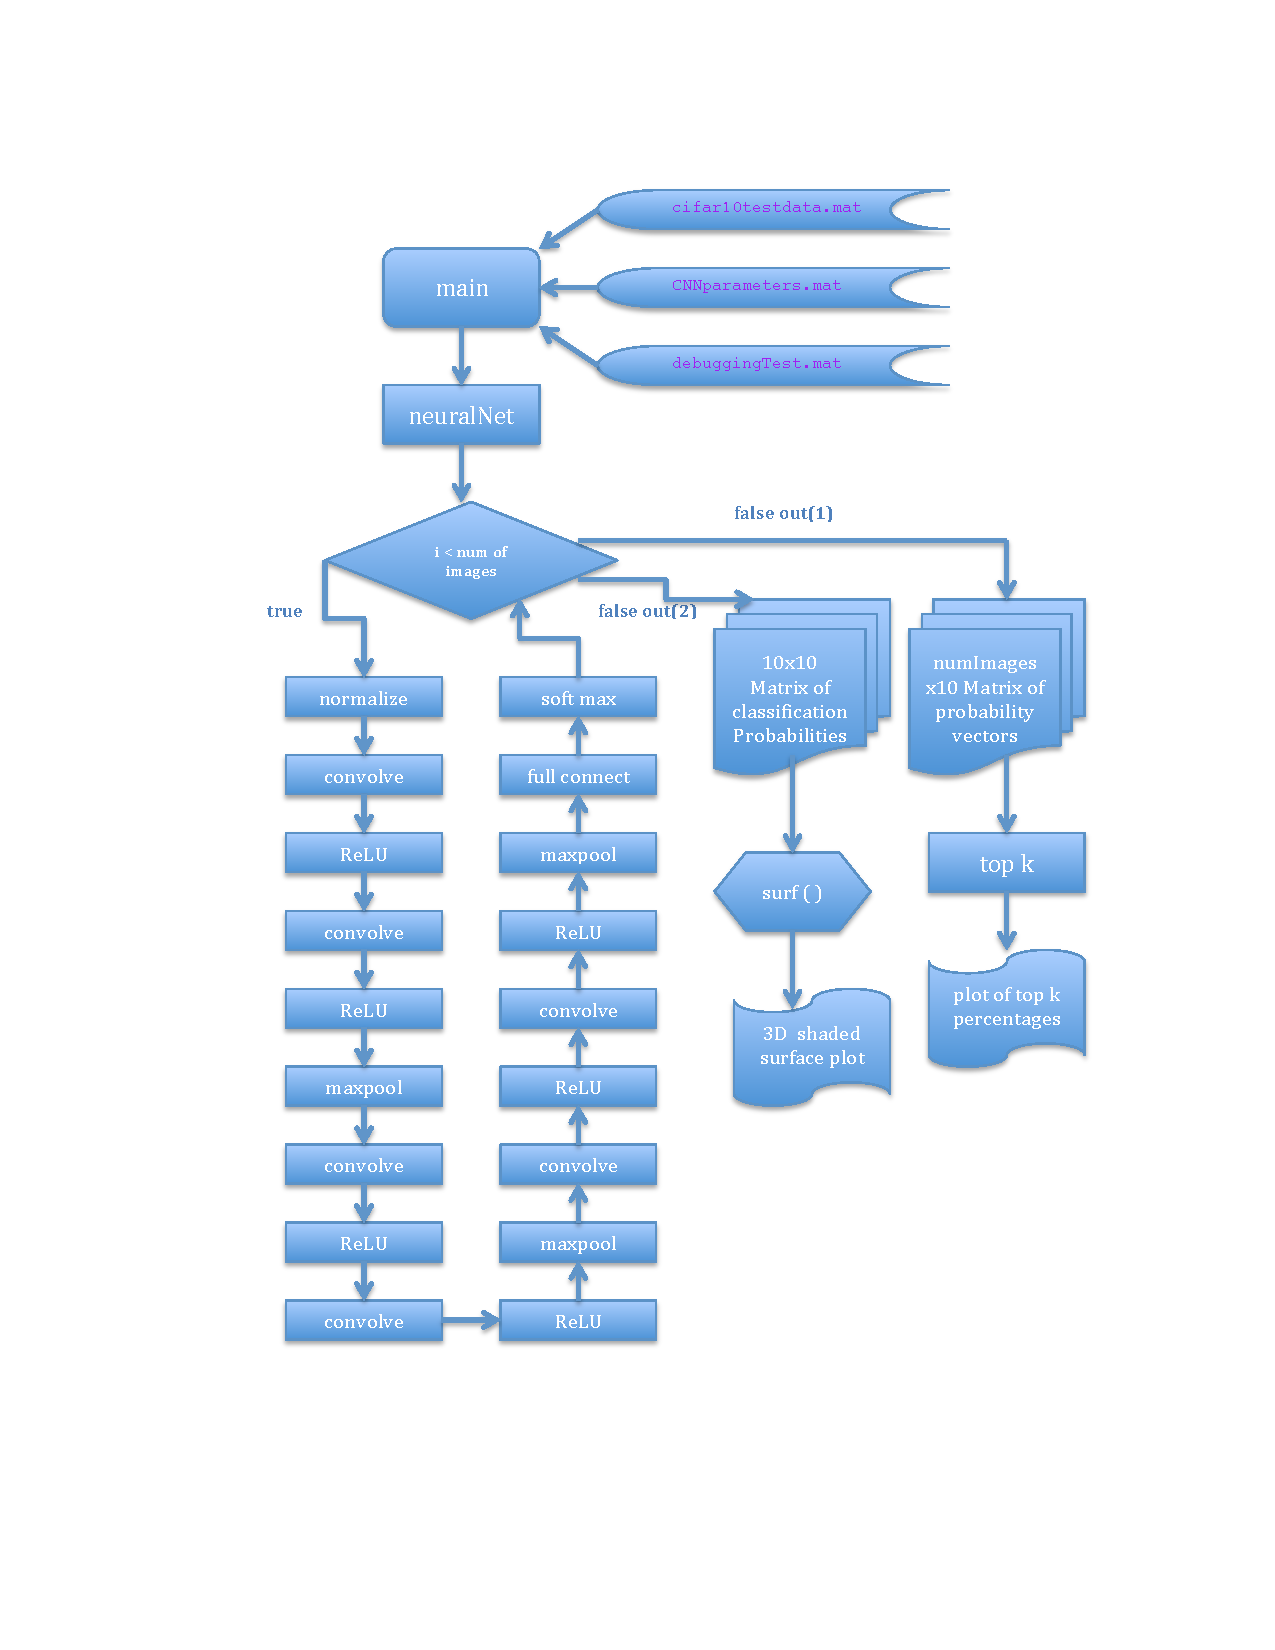
\includepdf[pages={1}]{../FlowChart_pdf_1b.pdf}

\section{Experimental Observations}

\subsection{Intermediate Output}

Intermediate output generated by the CNN is included in the appendix attached to this report.  Each figure shows the concatenated output of each layer as a gray scale image.  The images can be produced by running `demo.m.'

Observation of the output from each layer is consistent with the project description.  Normalization produces an image with scaled pixel values but is relatively unchanged.  Convolution produces a set of images with different feature sets extracted.  The ReLu produces an image with a 0 threshold (MATLAB's imagesc command slightly changes the output image because the range of the pixel values in the image changes).  Max Pooling reduces the size of the image by a factor of (nxn) and has the effect of making the previous image look more ``blocky'' via down-sampling.  Finally, we have the fully-connected layer and the soft max layer which produce a vector of classification probabilities from the image which are represented by the bar graph.

\section{Performance Evaluation}
\subsection{Results}
	The following results were the outcome of classifying images as the class associated with the highest probability in the probability vector.
\begin{center}
	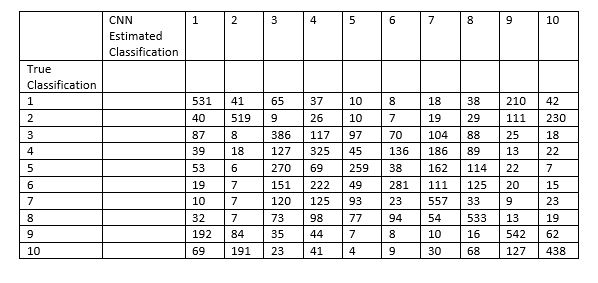
\includegraphics[scale=0.7]{confusionmatrix}
	~\\~\\
	
		\textbf{Accuracy = 43.7\%}
\end{center}


\begin{center}
	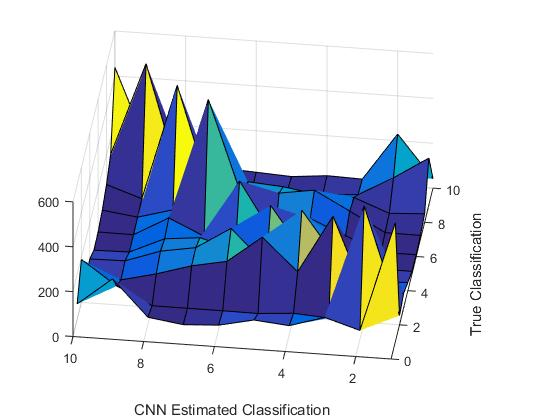
\includegraphics[scale=0.6]{confsurf}
	~\\~\\
\end{center}
\textbf{Discussion:}

	
   The surface plot above demonstrates how well the CNN classifies images. There is a very strong response on the diagonal which represents the correct classifications. What is interesting is that this matrix is somewhat diagonal. This demonstrates that if images in a class of images $C_1$ are being confused for images in a class of images $C_2$, then images in $C_2$ are also being confused for images in $C_1$. A lot of this confusion is entirely logical; for example, trucks and automobiles are frequently confused for each other. Another great example of confusion are cats and dogs are frequently confused for one another. We are again very impressed with how well the CNN because it not only detects similarities between images within a class, but it detects similarities amongst images spanning multiple classes.
       
    ~\\
    \noindent
    Note: The above results were produced using NeuralNet function located in 'NeuralNet.m'.

\subsection{Looking at the Top-k Highest Probabilities}
	The following subsection looks at how frequently an image's true class appears in one of the top-k ranked classes, as determined by probability scores sorted from highest to lowest.
\begin{center}
	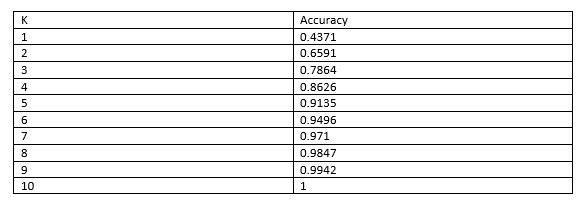
\includegraphics[scale=0.8]{topktable}

\end{center}
	Note: Accuracy is the percentage of times that the correct object class appeared in the top-k ranked classes, as determined by probability scores sorted form highest to lowest. 
	~\\
\begin{center}
	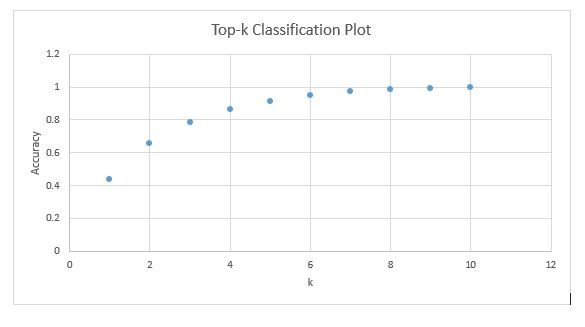
\includegraphics[scale=0.8]{topkplot}
	~\\~\\
\end{center}
\textbf{Discussion:}
      We were very surprised to see the top-k classification plot follow a logarithmic distribution. This demonstrates that the probability estimations provided by the CNN are accurate. We expected the probability estimations to be an arbitrary metric, used to find reasonable classification for an image, but looking at the logarithmic nature of the plot it is clear that the probabilities are very accurate. In fact, when looking at the probabilities for the 10,000 images you will find that on average an images top-k probabilities sum up to the y value shown above. For example, the average max probabilities for the 10,00 images is .4425 and 43.71\% of the time the max probability is correct. Even more interesting, the average of the top 2 probabilities added together for each image is .6646 and the chance of the true class being associated with one of the top two highest probabilities in its probability vector .6591, as shown above.

	~\\
	\noindent
	Note: The above results were produced using the topk function located in 'topk.m' and NeuralNet function located in 'NeuralNet.m'.

\section{Further Exploration}
\subsection{Test Cases}
To test the robustness/accuracy of the training outside of the given data set, additional test images were gathered and fed into the CNN.  Images were rescaled to thumbnail size (32x32x3) with the Matlab command
\begin{lstlisting}
thumbnail = imresize(img, [32 32]);
\end{lstlisting}

\noindent
110 images total were collected; 100 fell into the preexisting image classes, 10 contained scenes not falling into any preexisting class.  Running these new 10 images through the CNN yielded the following results:\\

\begin{tabular}{ | c | c | c |}
  \hline
  Image \# & Image Contents & CNN Classification \\
  \hline		
  Image 1 & Tree in Field & Horse (8) \\
  Image 2 & Winter Mountain Scene & Ship (9) \\
  Image 3 & Ryan and Zach & Bird (3) \\
  Image 4 & Steve & Frog (7) \\
  Image 5 & Sean & Cat (4) \\
  Image 6 & Desktop Computer & Automobile (2) \\
  Image 7 & Football on Field & Deer(5) \\
  Image 8 & Robert Collins & Truck (10) \\
  Image 9 & Old Main & Bird(3) \\
  Image 10 & Penn State Logo & Truck (10)\\
  \hline  
\end{tabular}

~\\~\\
\noindent
All of the exploratory images we used were either taken by us or were taken from Google Images. The code we used to read in the exploratory images can be found in 'getAllFiles.m' and 'getTrueClass.m'. We produced the results above by running the 10 images through the function found in 'NeuralNet.m' and classifying the images by assigning the image the class associated with the highest probability. The classification process was done manually.

\subsection{Reclassification}
An attempt was made to distinguish these 10 images from the rest of the data set (i.e. reclassify these 10 images as unknown).  Let $V$ be the vector of output probabilities from the CNN for each image.  Let $C$ be the classification of the image producing probability vector $V$.  Originally, we have\\~\\
\begin{math}
p_i \in V \\
p_{max} = \max(p_1, p_2,...,p_{10}) \\
C = i $ given $ p_i = p_{max}
\end{math}

~\newline\noindent
To reclassify the images we use\\
\noindent
\begin{math}
p_{max} = \max(p_1,p_2,...,p_{10}) \\
P = \{p_1,p_2,...,p_{10}\} \setminus \{p_{max}\} \\
p_{2max} = \max(P) \\~\\
\begin{cases}
C = i $ given $ p_i = p_{max} & $for	$ p_{max} - p_{2max} >= 0.25 \\
C = 11 & $otherwise$
\end{cases}
\end{math}
~\\~\\
Less precisely, the difference between the two peak responses was thresholded by .25; so, if there were two strong responses, the image is reclassified as unknown.
~\\~\\
The code used to reclassify images can be found in 'identify\_exploratory.m'.
\subsection{Results After Reclassification}
In the confusion matrix below, classes 1 through 10 are the same classifications.  Class 11 identifies an unknown image class. \\\\
\begin{tabular}{ | c | c | c | c | c | c | c | c | c | c | c | c | c | }
\hline
	 & CNN
Class & 1 & 2 & 3 & 4 & 5 & 6 & 7 & 8 & 9 & 10 & 11 \\ \hline
	True 
Class &  &  &  &  &  &  &  &  &  &  &  &  \\ \hline
	1 &  & 3 & 0 & 0 & 0 & 0 & 0 & 0 & 0 & 1 & 0 & 6 \\ \hline
	2 &  & 1 & 2 & 0 & 0 & 0 & 0 & 0 & 0 & 2 & 0 & 5 \\ \hline
	3 &  & 1 & 0 & 2 & 0 & 0 & 0 & 0 & 0 & 0 & 0 & 7 \\ \hline
	4 &  & 0 & 0 & 0 & 1 & 0 & 0 & 0 & 0 & 0 & 0 & 9 \\ \hline
	5 &  & 0 & 0 & 0 & 0 & 0 & 0 & 0 & 1 & 0 & 0 & 9 \\ \hline
	6 &  & 0 & 0 & 2 & 0 & 0 & 0 & 0 & 0 & 0 & 0 & 8 \\ \hline
	7 &  & 0 & 0 & 0 & 1 & 0 & 0 & 1 & 0 & 0 & 0 & 8 \\ \hline
	8 &  & 0 & 0 & 1 & 1 & 0 & 0 & 1 & 4 & 0 & 0 & 3 \\ \hline
	9 &  & 0 & 0 & 0 & 0 & 0 & 0 & 0 & 0 & 5 & 0 & 5 \\ \hline
	10 &  & 0 & 0 & 0 & 0 & 0 & 0 & 0 & 0 & 0 & 5 & 5 \\ \hline
	11 &  & 0 & 0 & 0 & 0 & 0 & 0 & 0 & 0 & 1 & 0 & 9 \\ \hline
\end{tabular}

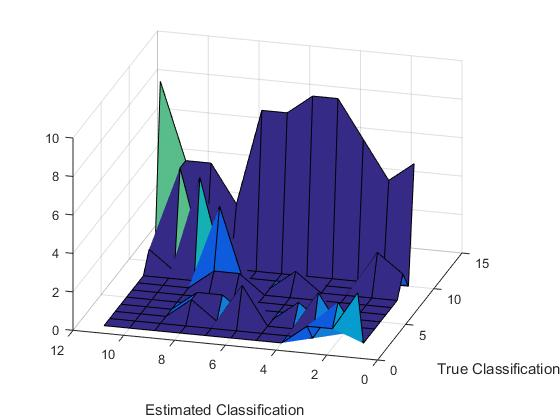
\includegraphics[scale=0.6]{confexp}
~\\~\\
\textbf{Accuracy = 29.09\%}
\\
The reclassification metric does well in placing the 10 new images in the unknown category, but it also incorrectly classifies many images as unknown.  Other metrics tested were:
\begin{enumerate}
\item Thresholding on the number of classes that had a response above 0.1 (the mean value for random classification)
\item Taking the spatial derivative of the probability vector; this metric actually produces zero-mean Gaussian noise with a very small standard deviation.
\end{enumerate}

~\\~\\
The code used to produce the results found in this section can be found in 'exploratory\_main.m'.

\section{Member Contributions}
	Overall the contributions made form each team member were pretty even. Whenever the team met to work on the project most of the team members were in attendance. Everyone who was in attendance at each team meeting attempted to work on a different piece of the project to ensure that we were making steady progress. The coding was not split up evenly as one team member did not attend the initial meeting and as a result he missed most of the actual coding and basically all of the design decisions. We attempted to split the report up evenly, but as the deadline approached scheduling meetings became difficult and some individuals were unavailable to work on the report. In conclusion, the work was not split up evenly among our four group members, but everyone attempted to contribute.

\newpage
\begin{appendices}
\section{Intermediate Output}

\begin{figure}[h!]
  \caption{Original Image}
  \centering
    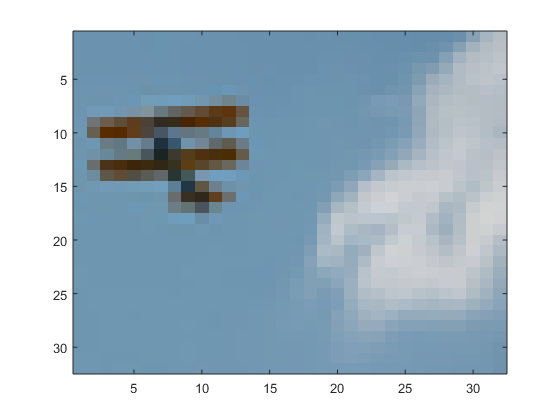
\includegraphics[width=0.75\textwidth]{layer/0}
\end{figure}

\begin{figure}[h!]
  \caption{Layer 1 Output}
  \centering
    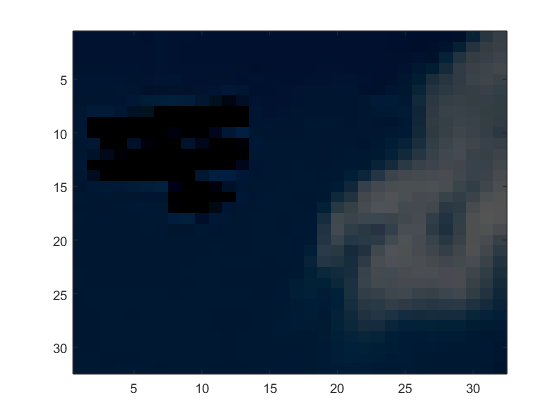
\includegraphics[width=0.75\textwidth]{layer/1}
\end{figure}

\begin{figure}[h!]
  \caption{Layer 2 Output}
  \centering
    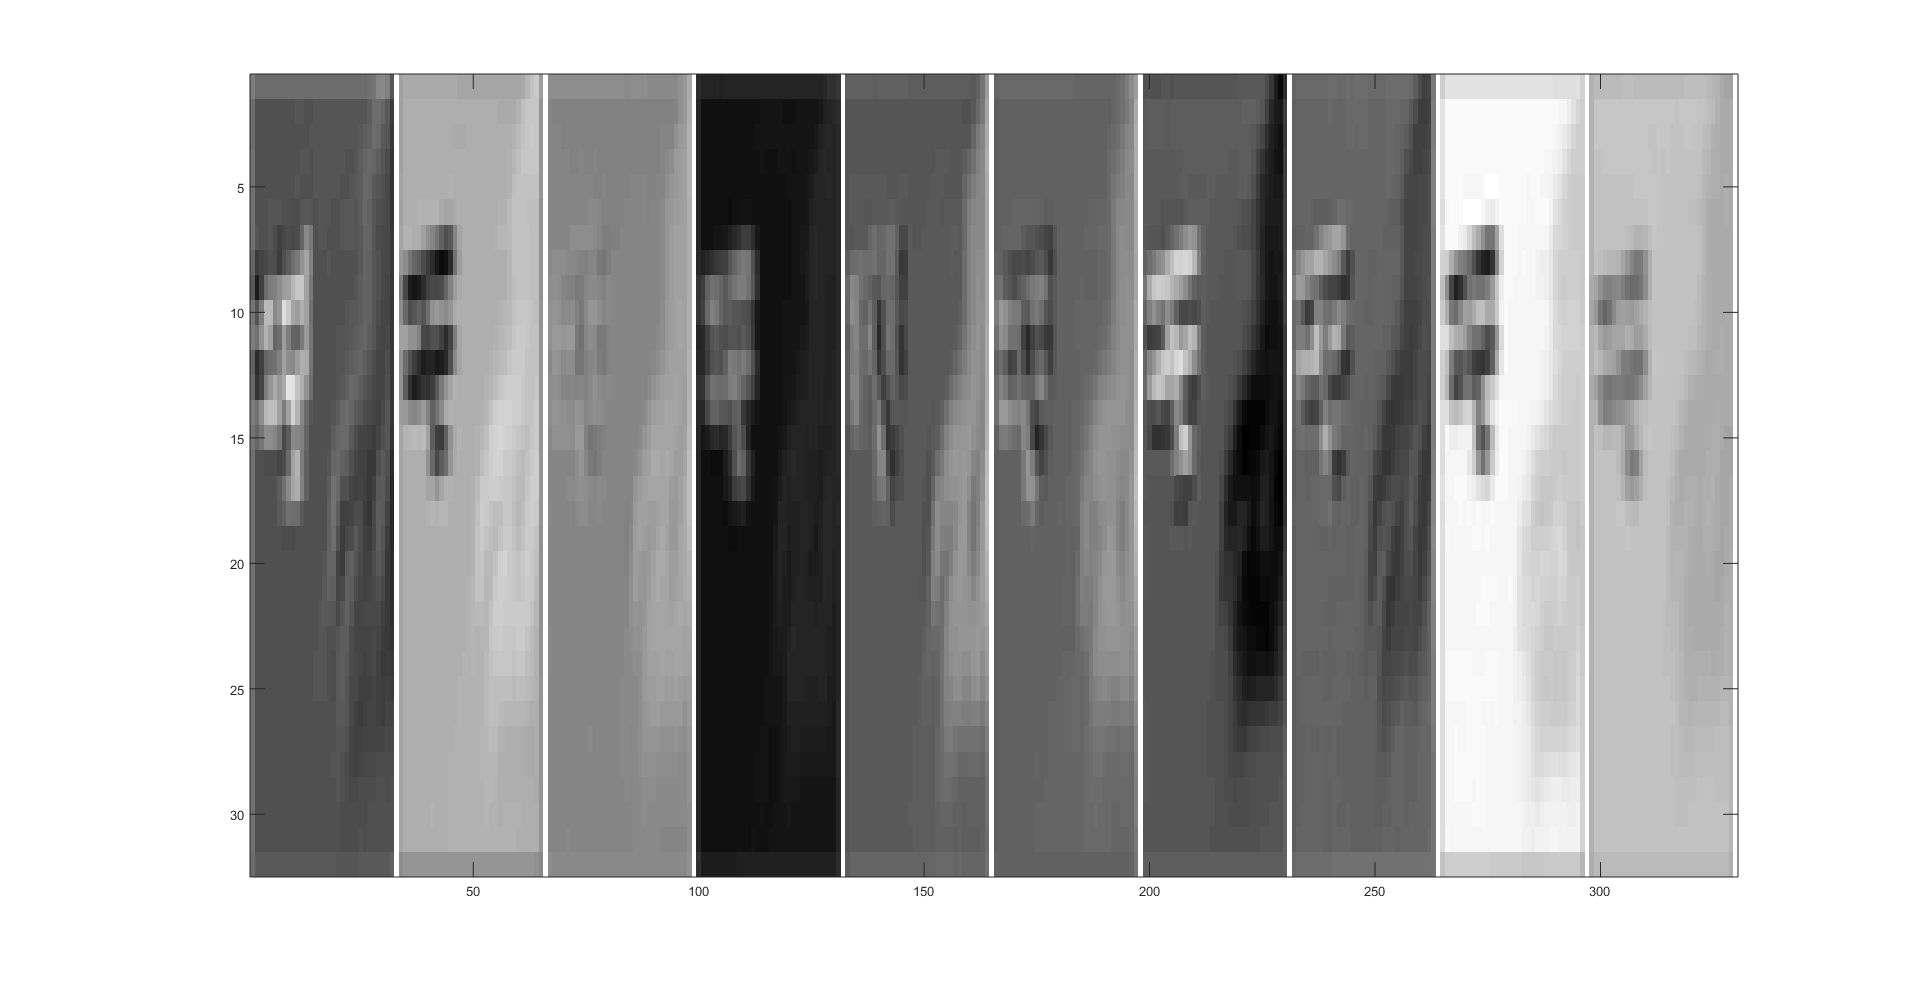
\includegraphics[width=\textwidth]{layer/2}
\end{figure}

\begin{figure}[h!]
  \caption{Layer 3 Output}
  \centering
    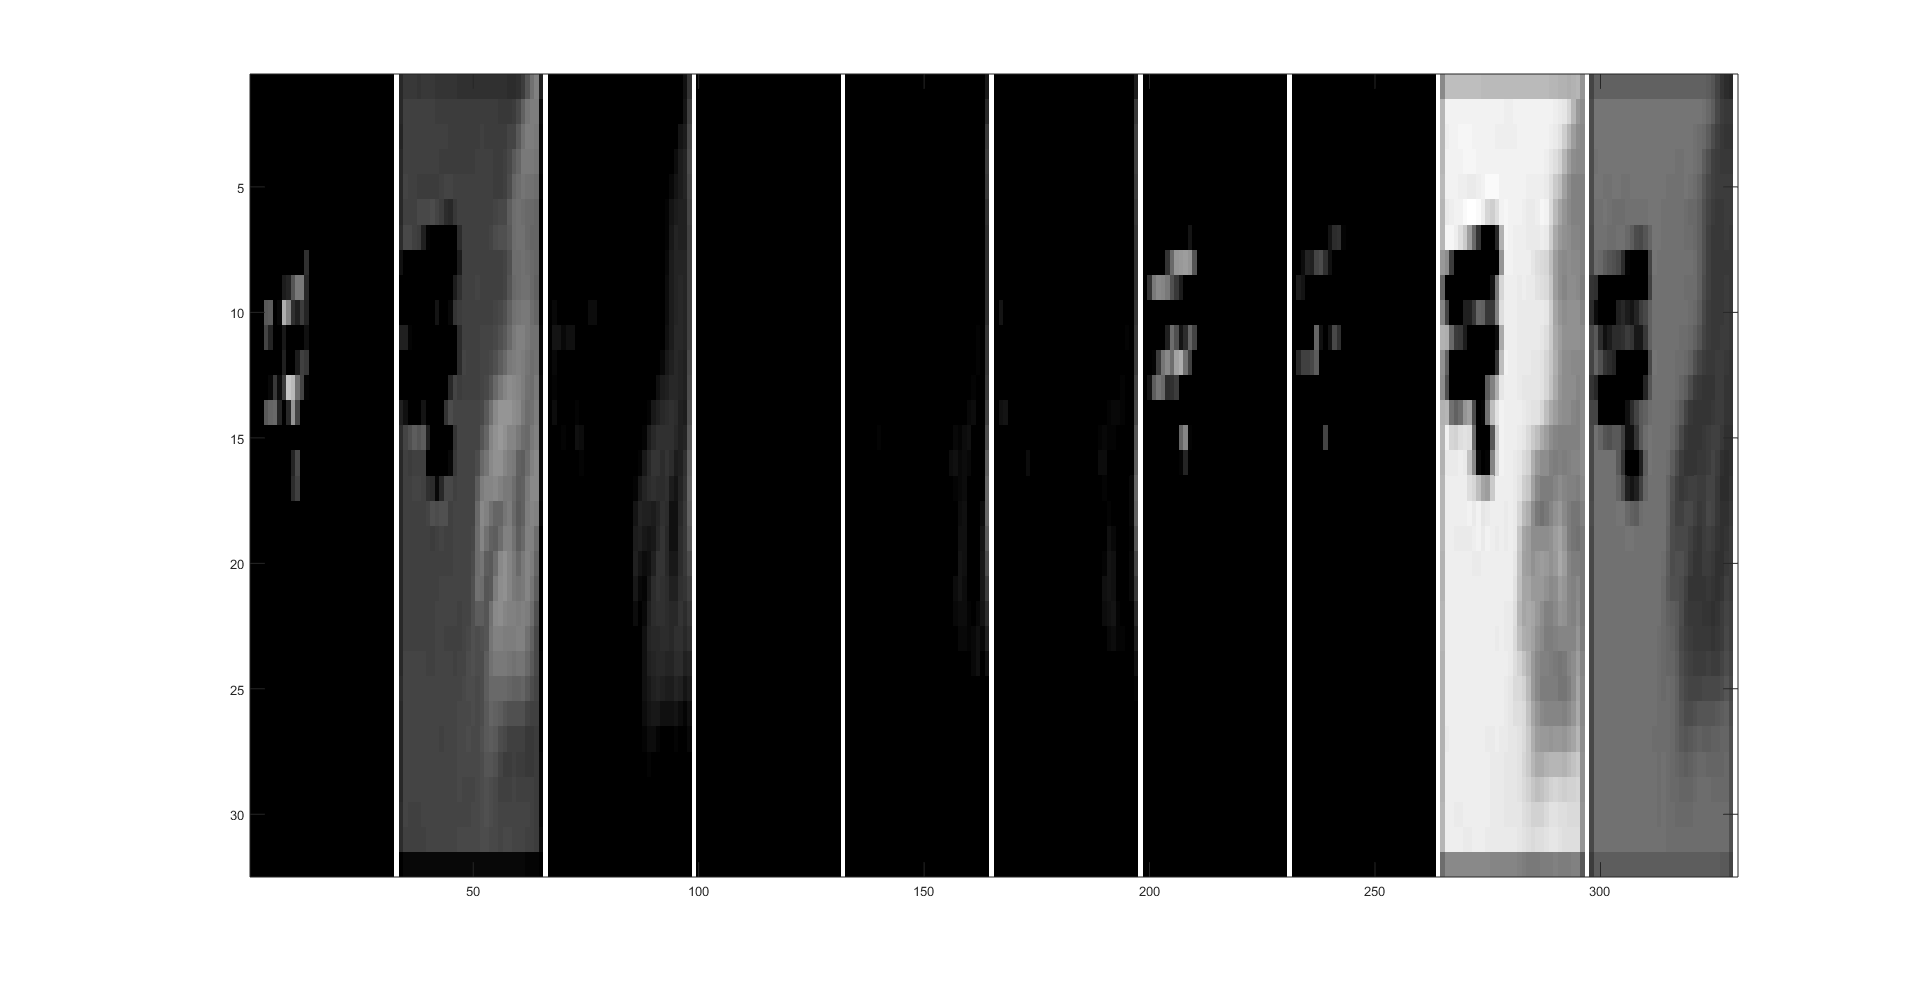
\includegraphics[width=\textwidth]{layer/3}
\end{figure}

\begin{figure}[h!]
  \caption{Layer 4 Output}
  \centering
    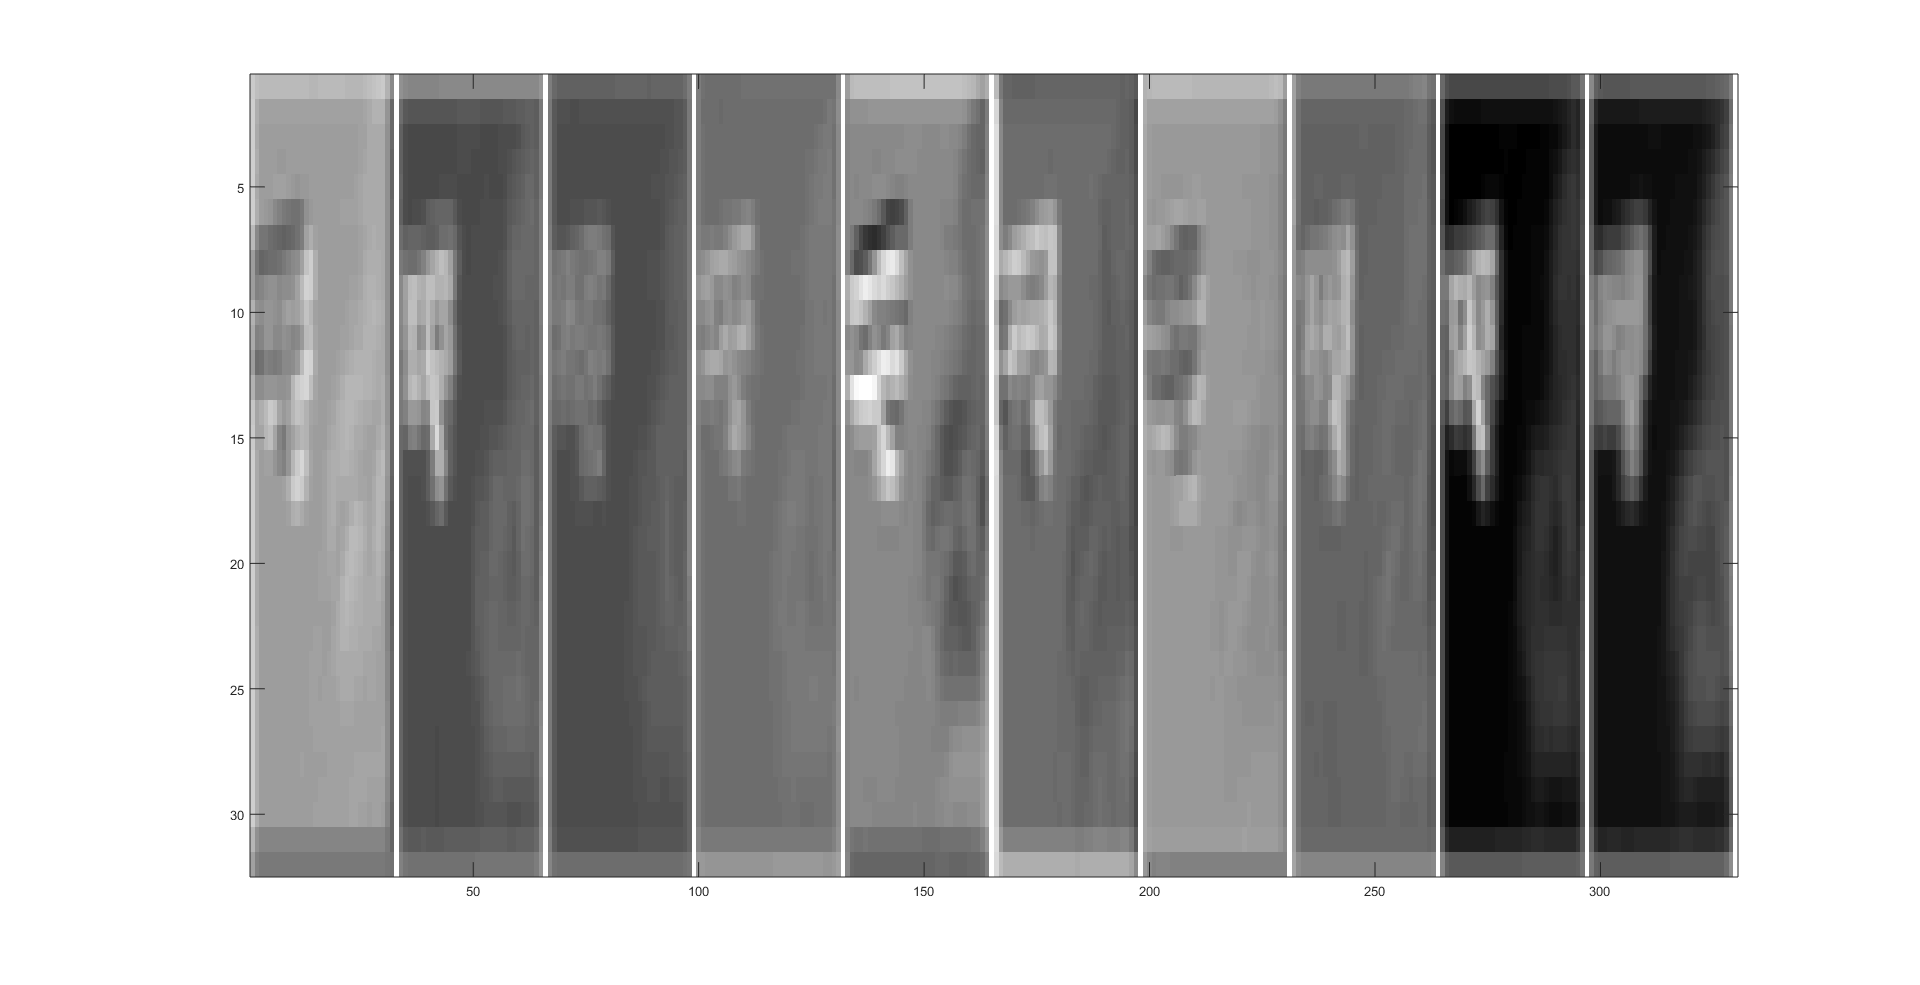
\includegraphics[width=\textwidth]{layer/4}
\end{figure}

\begin{figure}[h!]
  \caption{Layer 5 Output}
  \centering
    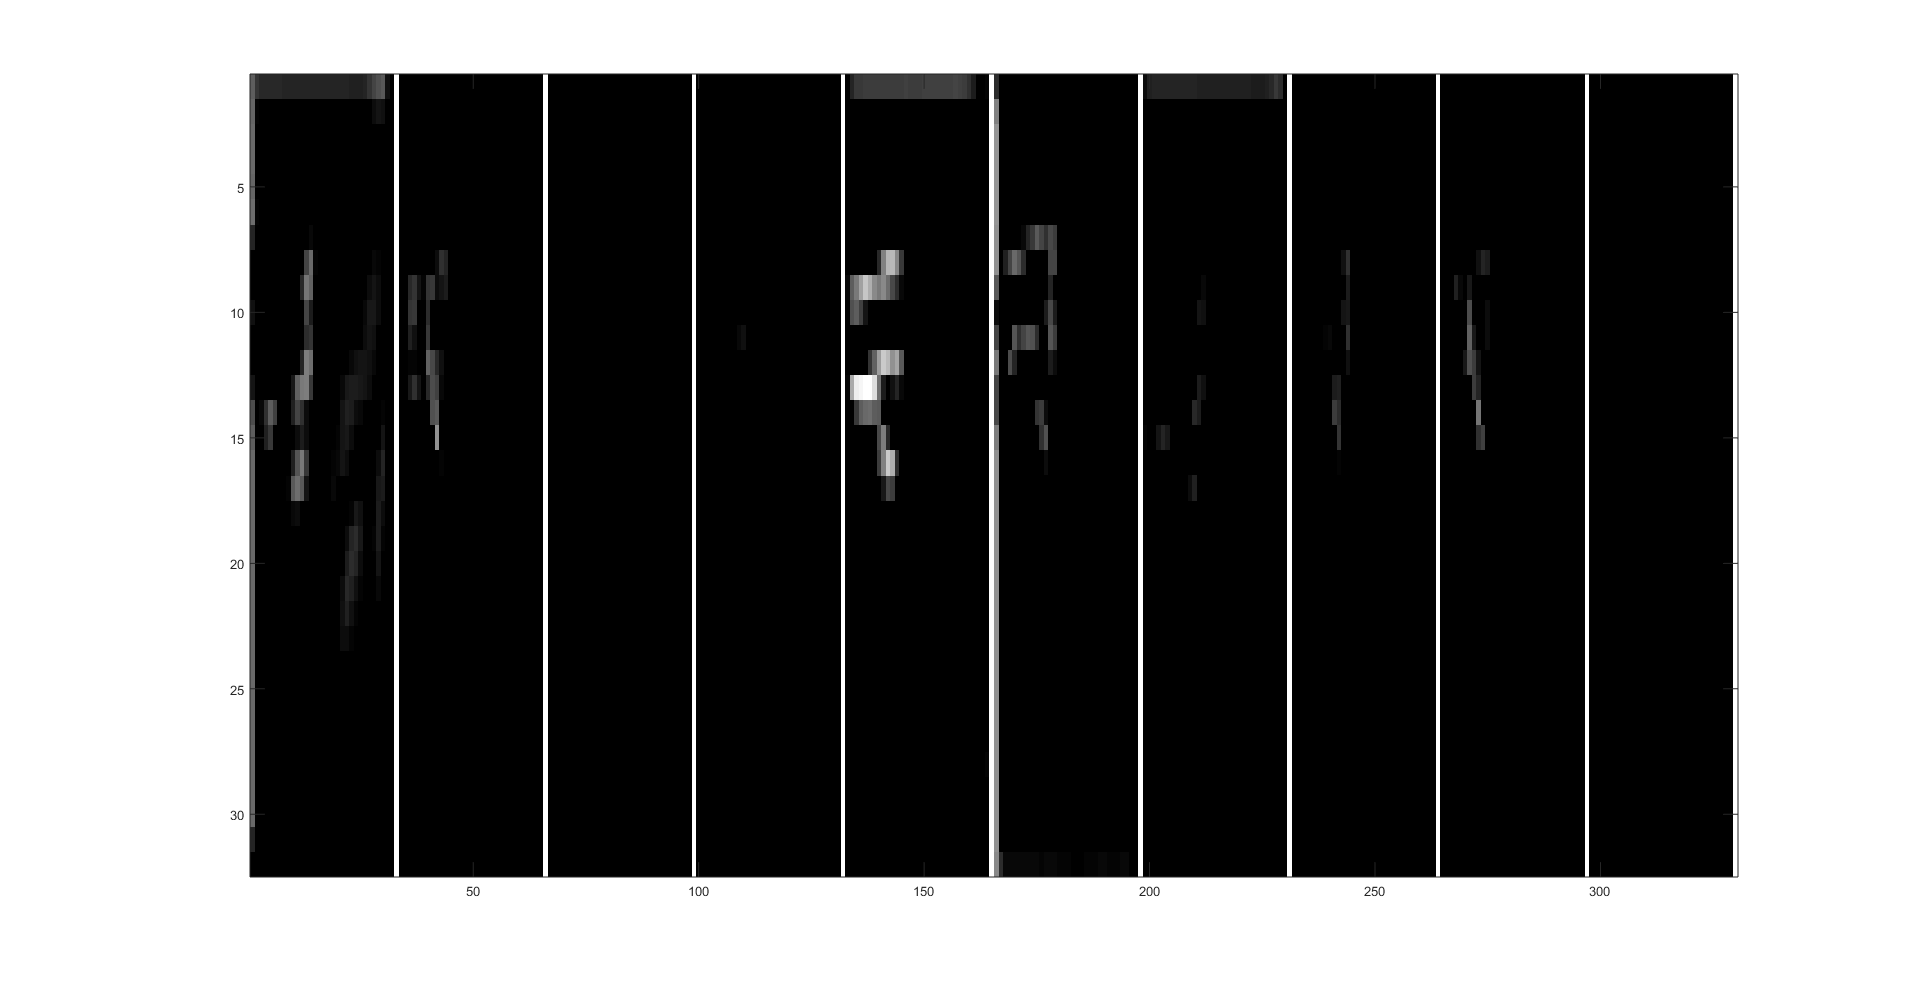
\includegraphics[width=\textwidth]{layer/5}
\end{figure}

\begin{figure}[h!]
  \caption{Layer 6 Output}
  \centering
    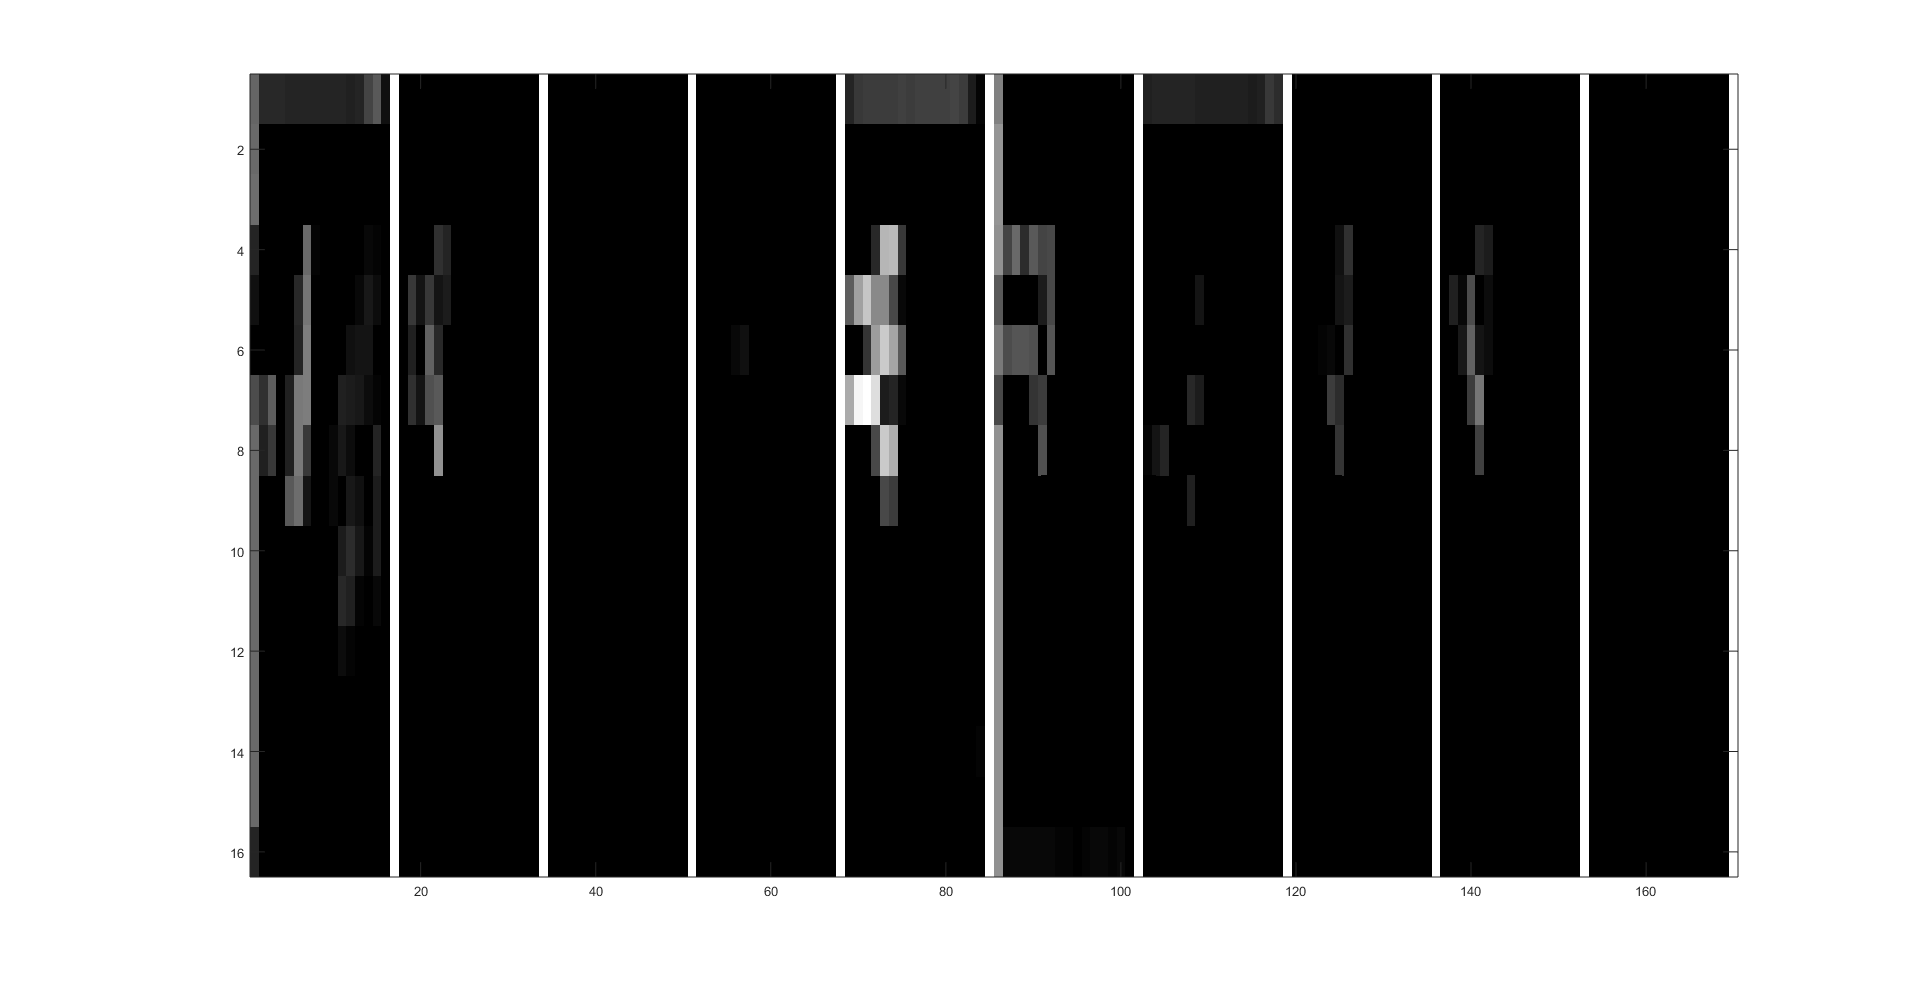
\includegraphics[width=\textwidth]{layer/6}
\end{figure}

\begin{figure}[h!]
  \caption{Layer 7 Output}
  \centering
    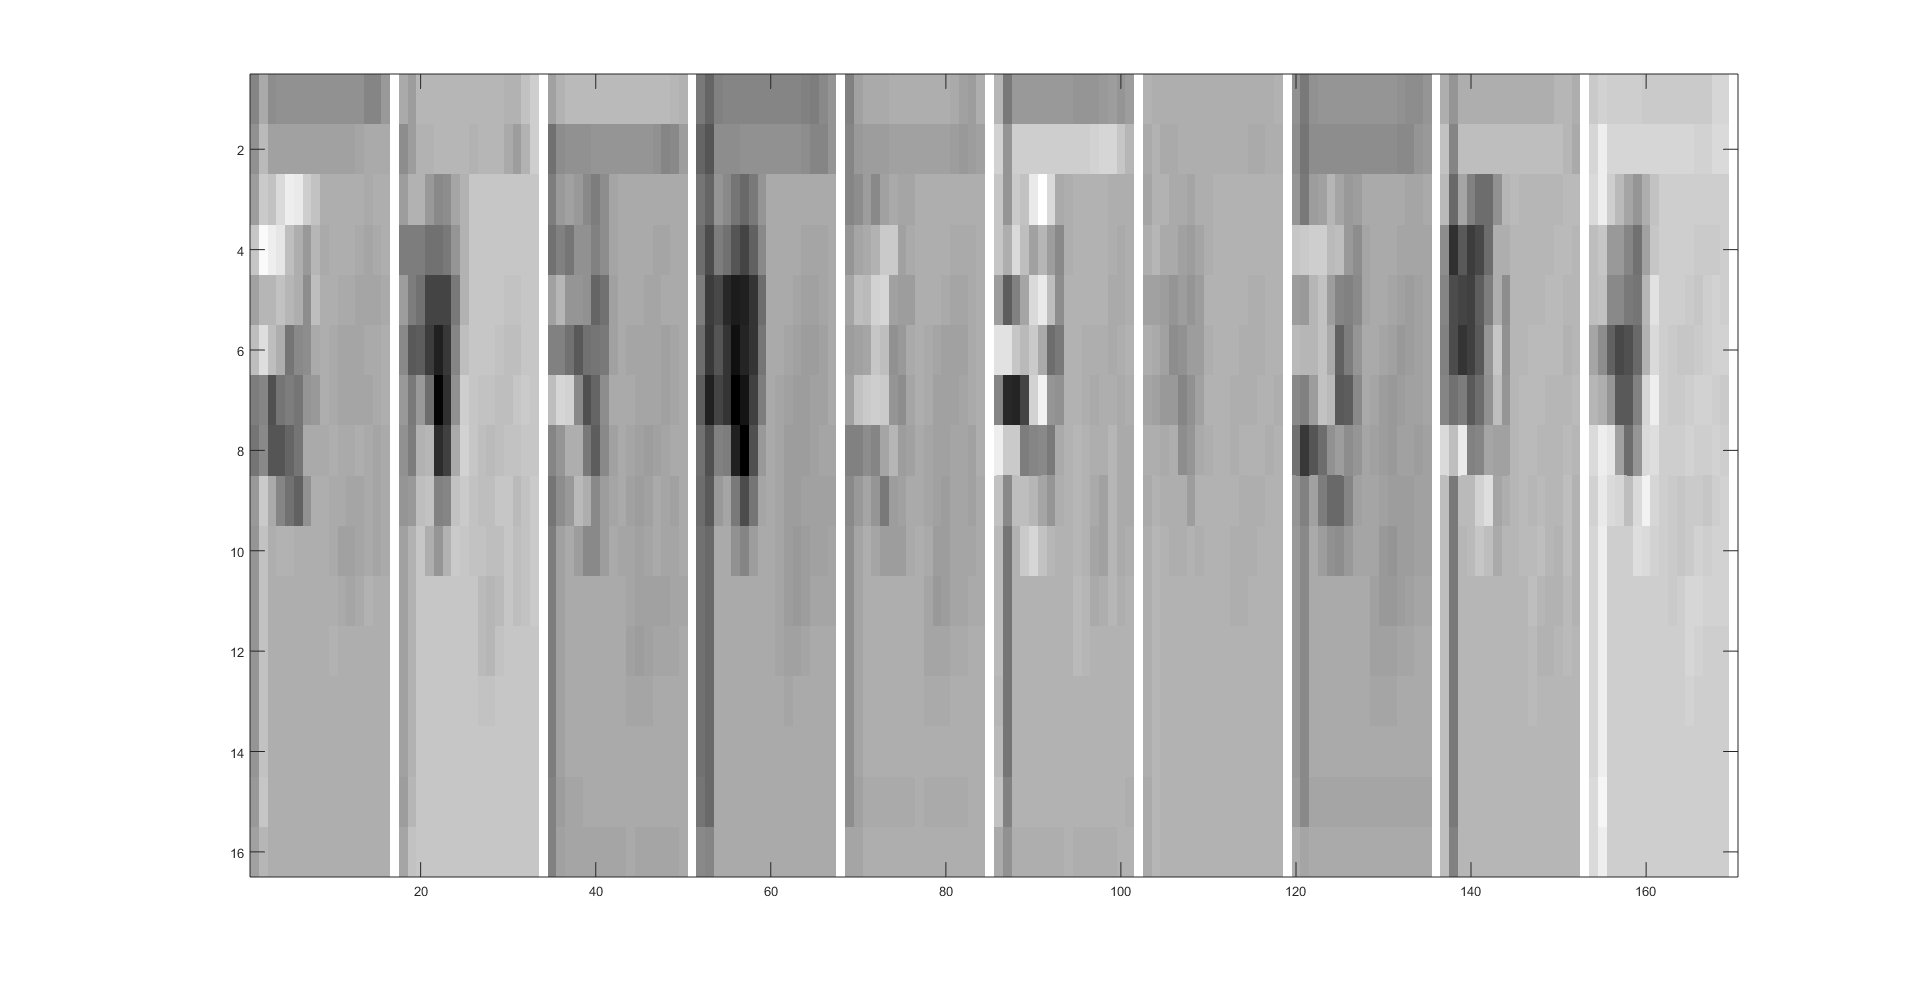
\includegraphics[width=\textwidth]{layer/7}
\end{figure}

\begin{figure}[h!]
  \caption{Layer 8 Output}
  \centering
    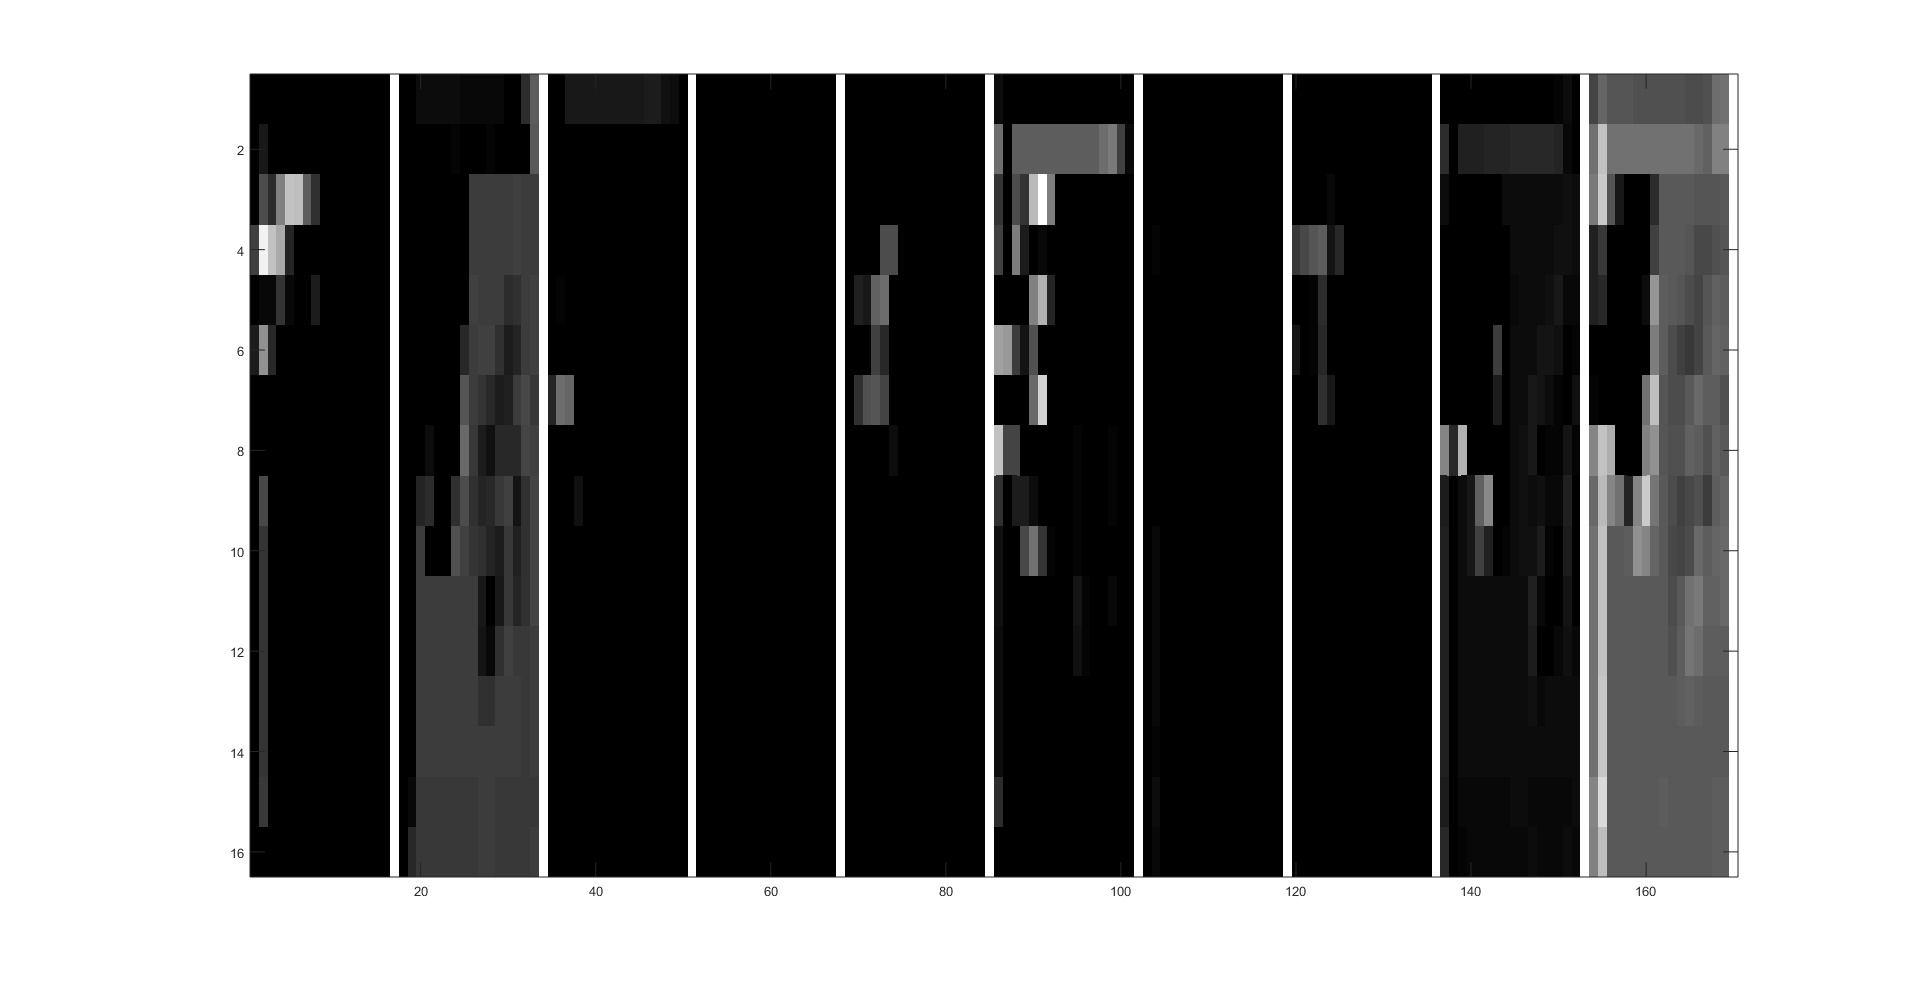
\includegraphics[width=\textwidth]{layer/8}
\end{figure}

\begin{figure}[h!]
  \caption{Layer 9 Output}
  \centering
    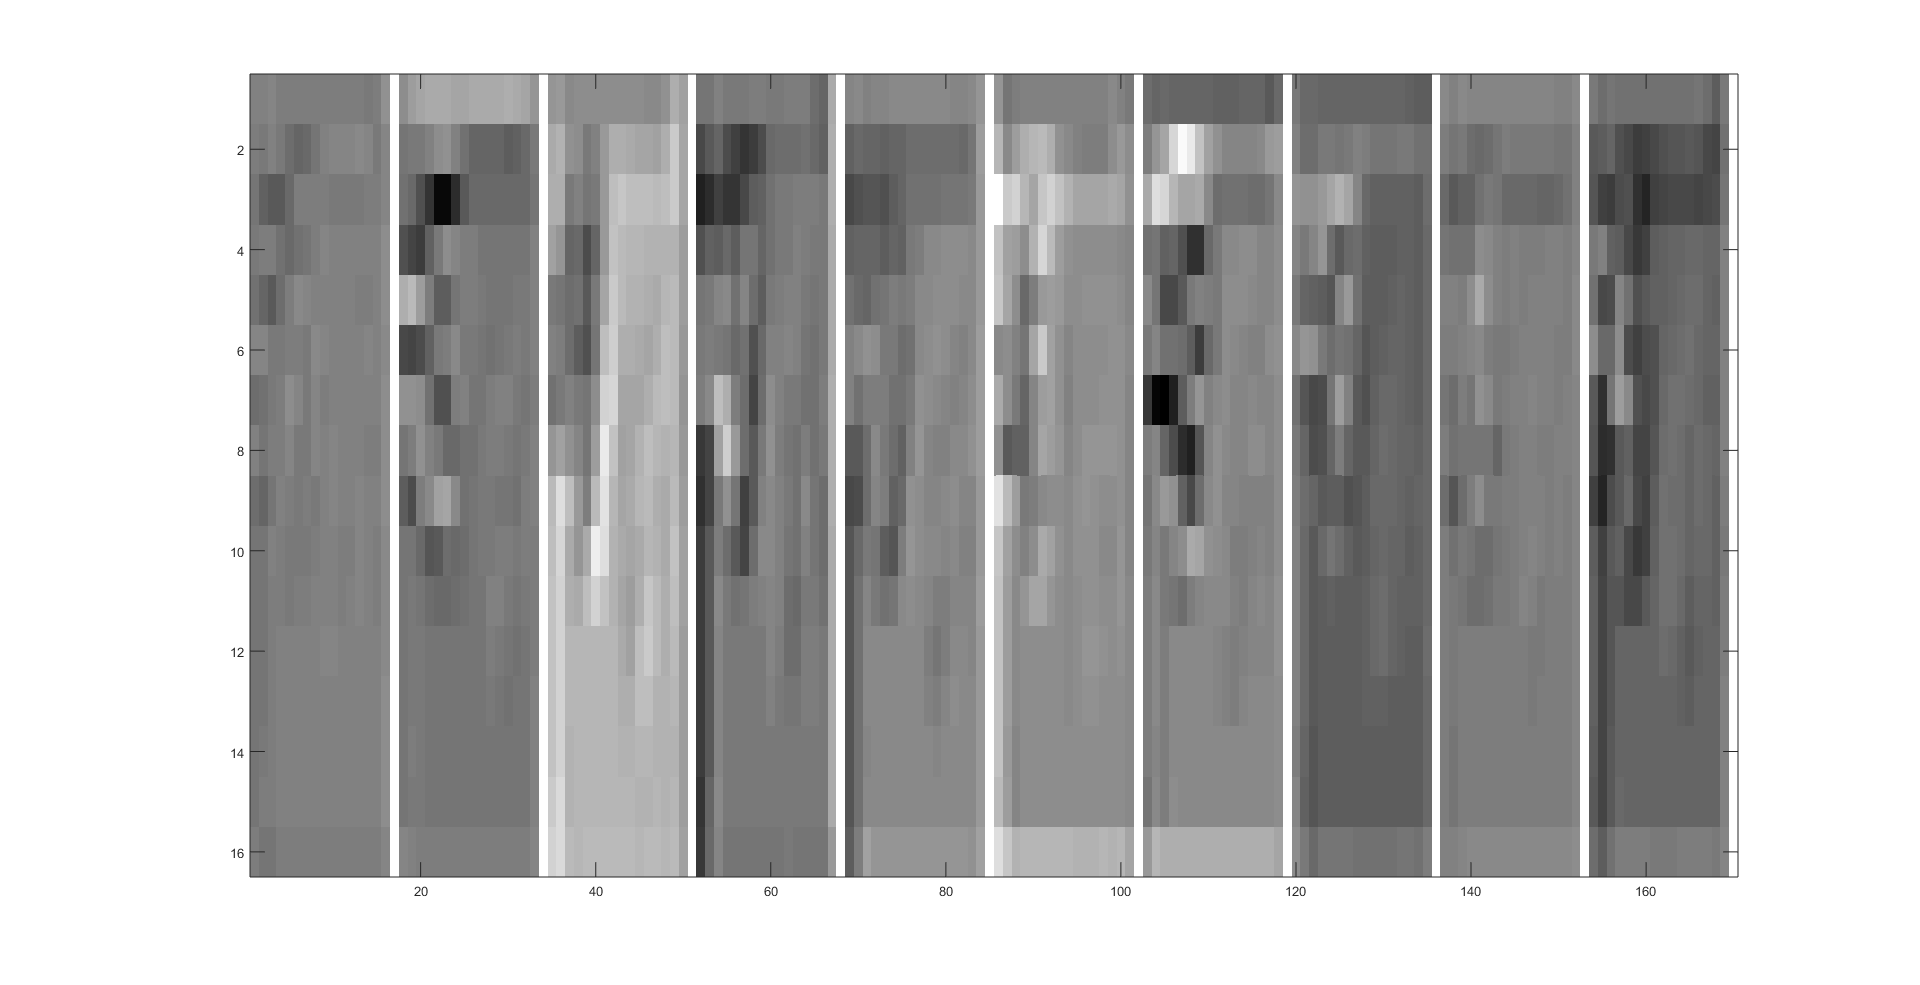
\includegraphics[width=\textwidth]{layer/9}
\end{figure}

\begin{figure}[h!]
  \caption{Layer 10 Output}
  \centering
    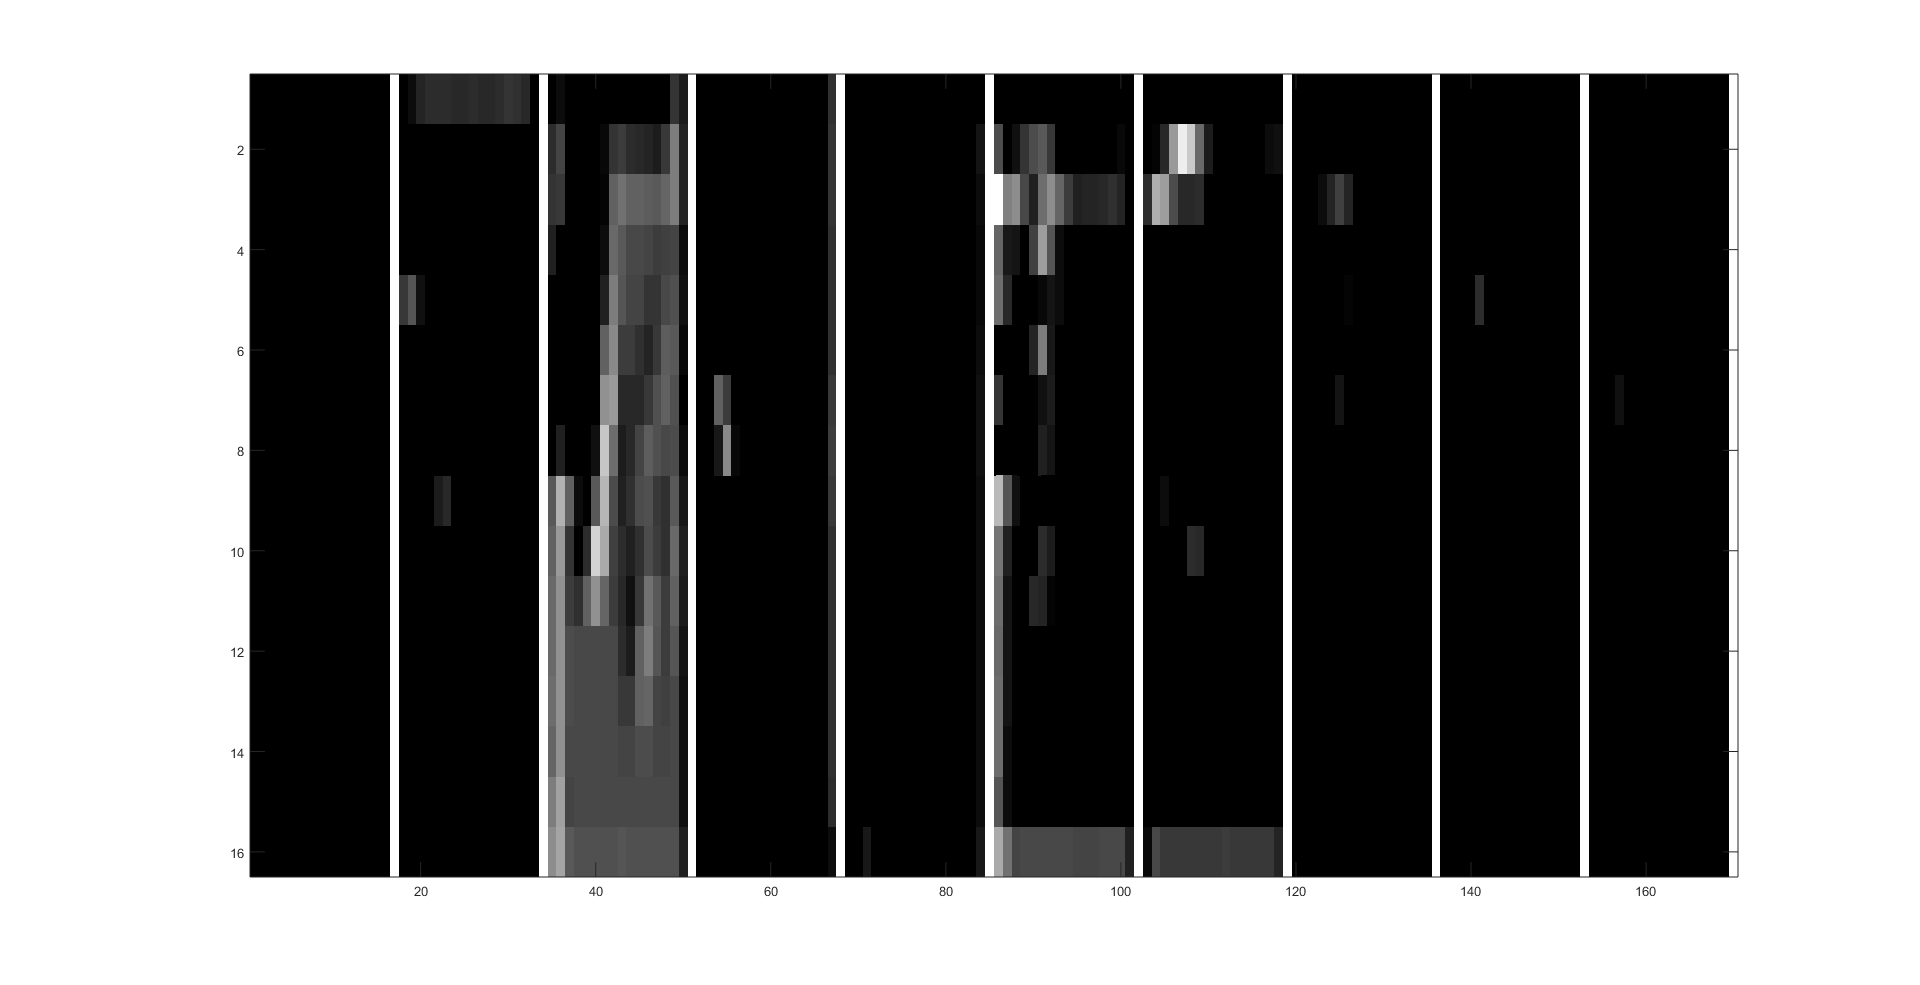
\includegraphics[width=\textwidth]{layer/10}
\end{figure}

\begin{figure}[h!]
  \caption{Layer 11 Output}
  \centering
    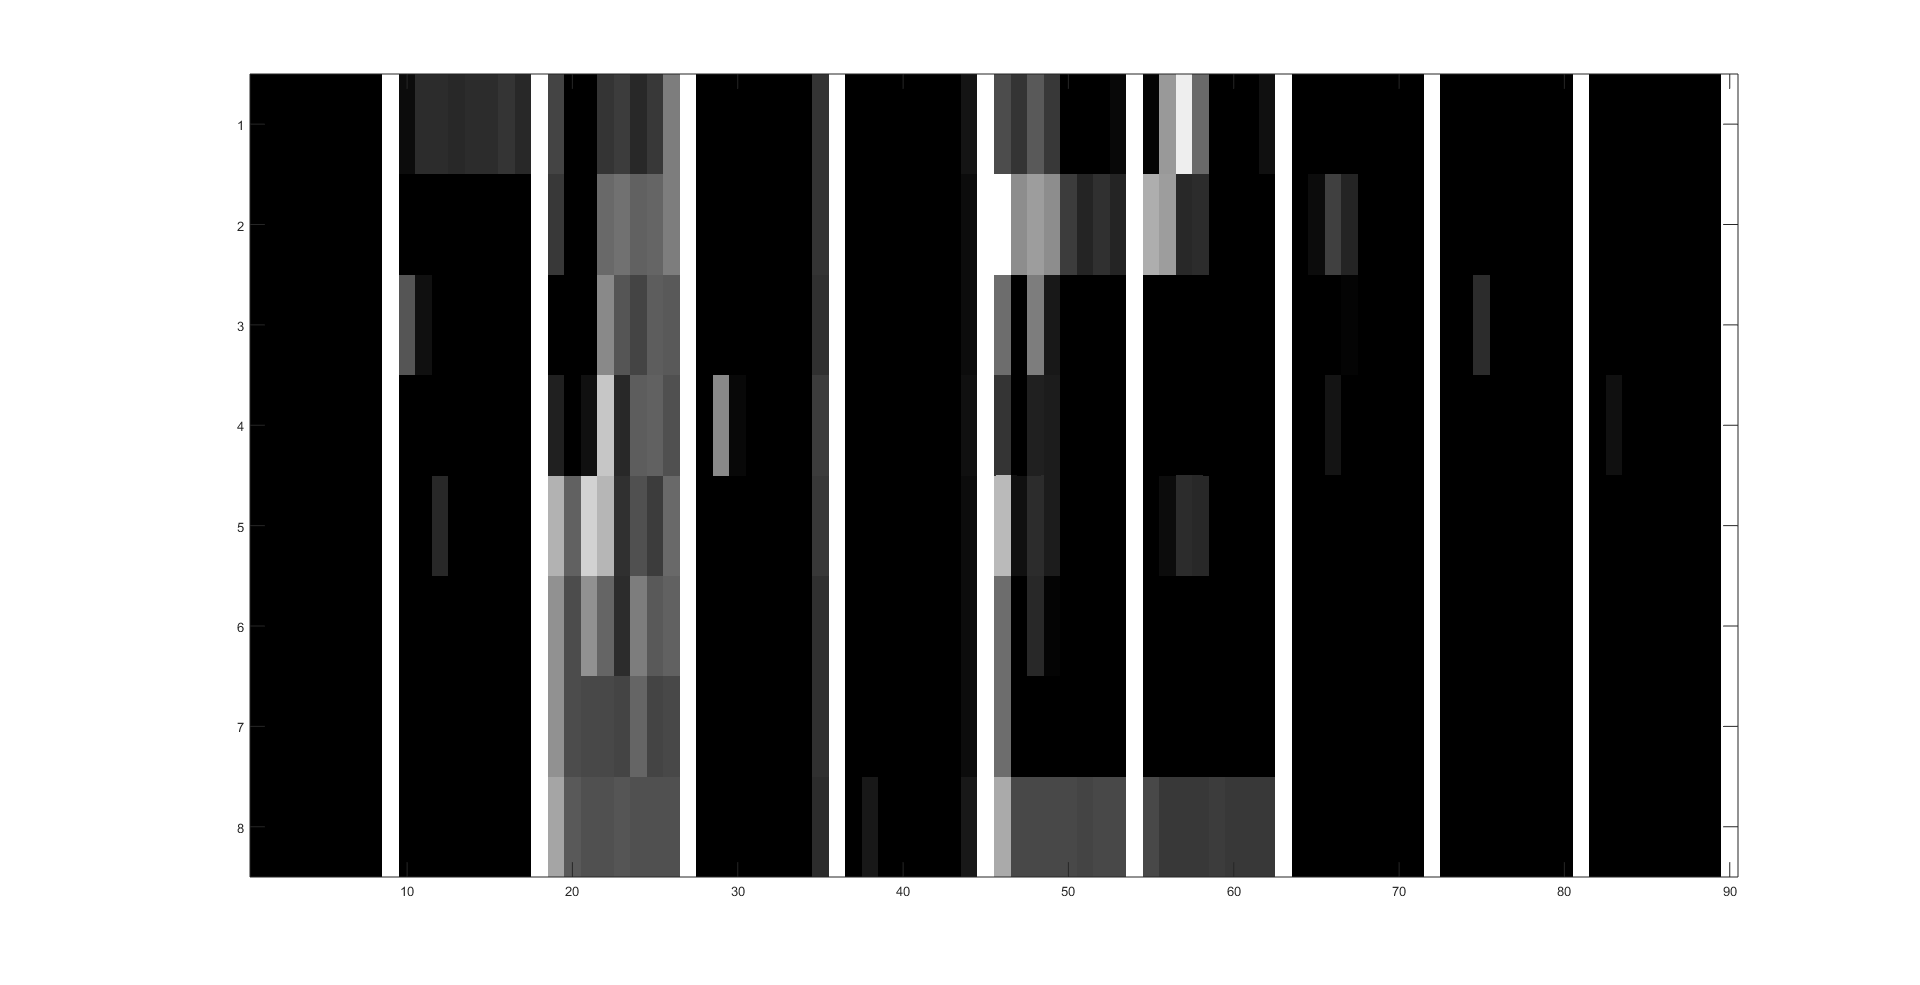
\includegraphics[width=\textwidth]{layer/11}
\end{figure}

\begin{figure}[h!]
  \caption{Layer 12 Output}
  \centering
    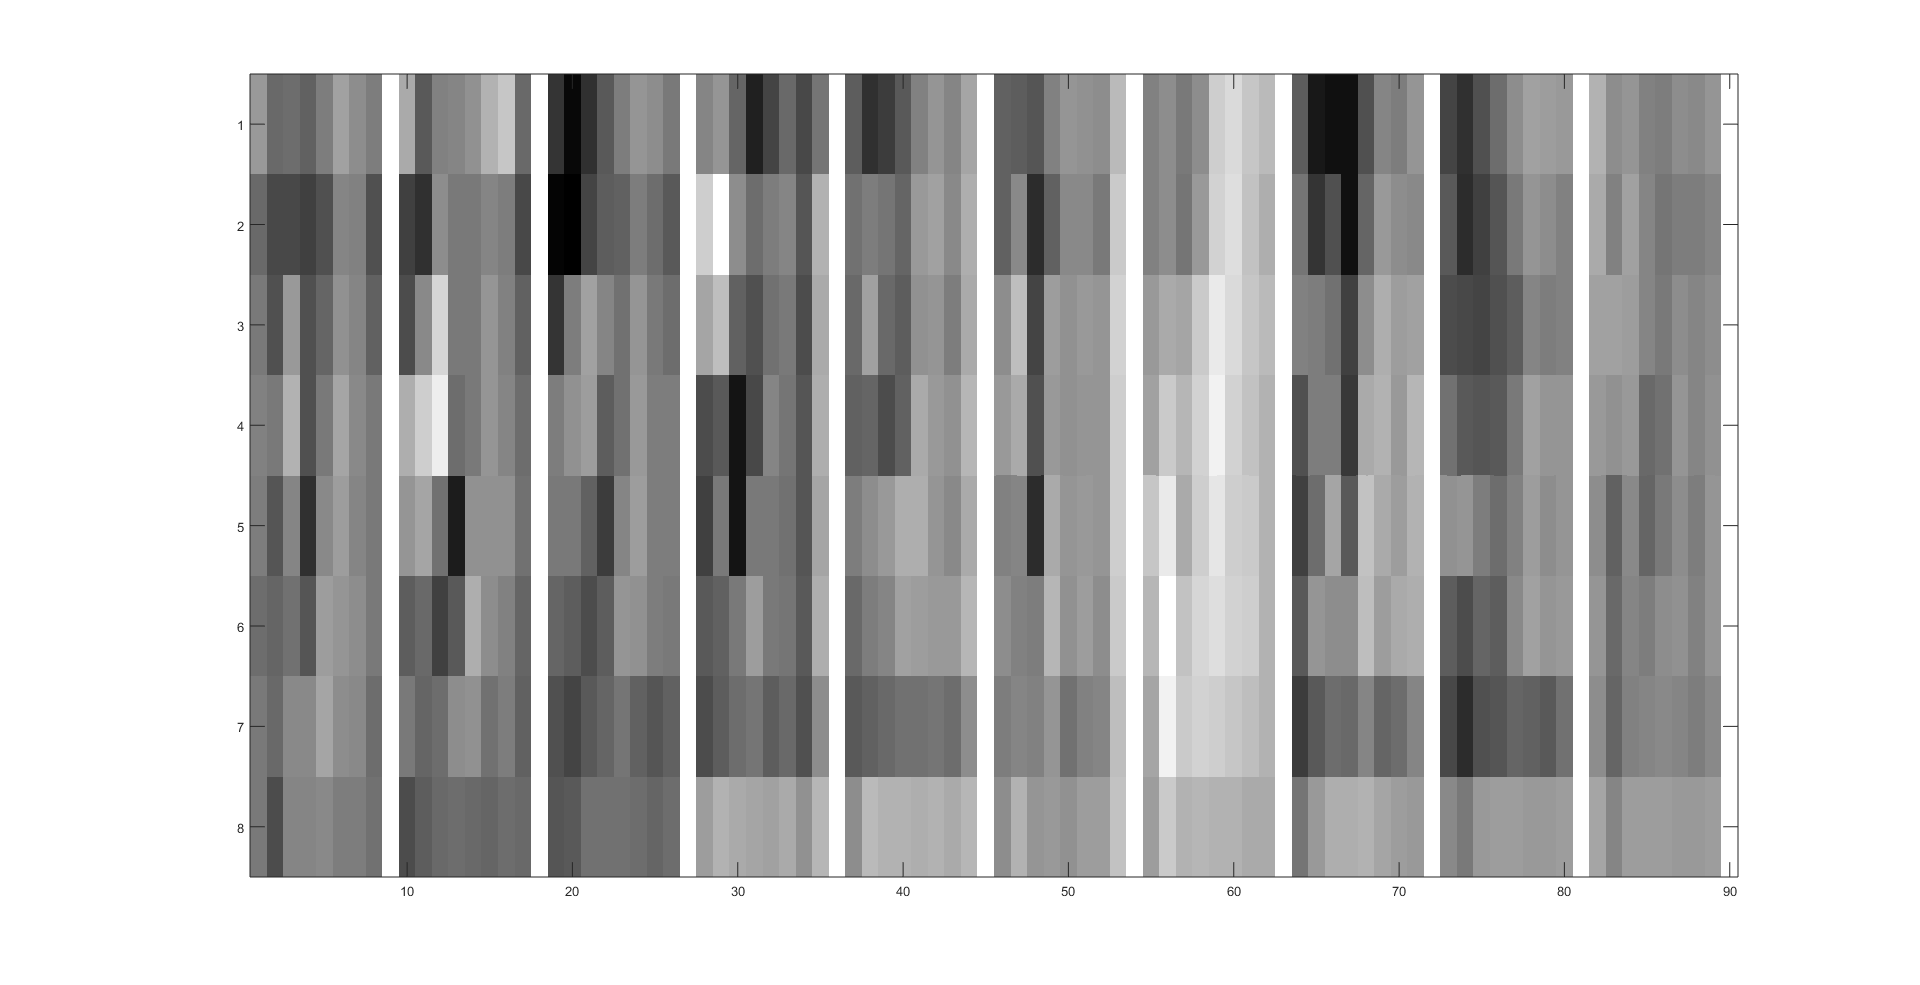
\includegraphics[width=\textwidth]{layer/12}
\end{figure}

\begin{figure}[h!]
  \caption{Layer 13 Output}
  \centering
    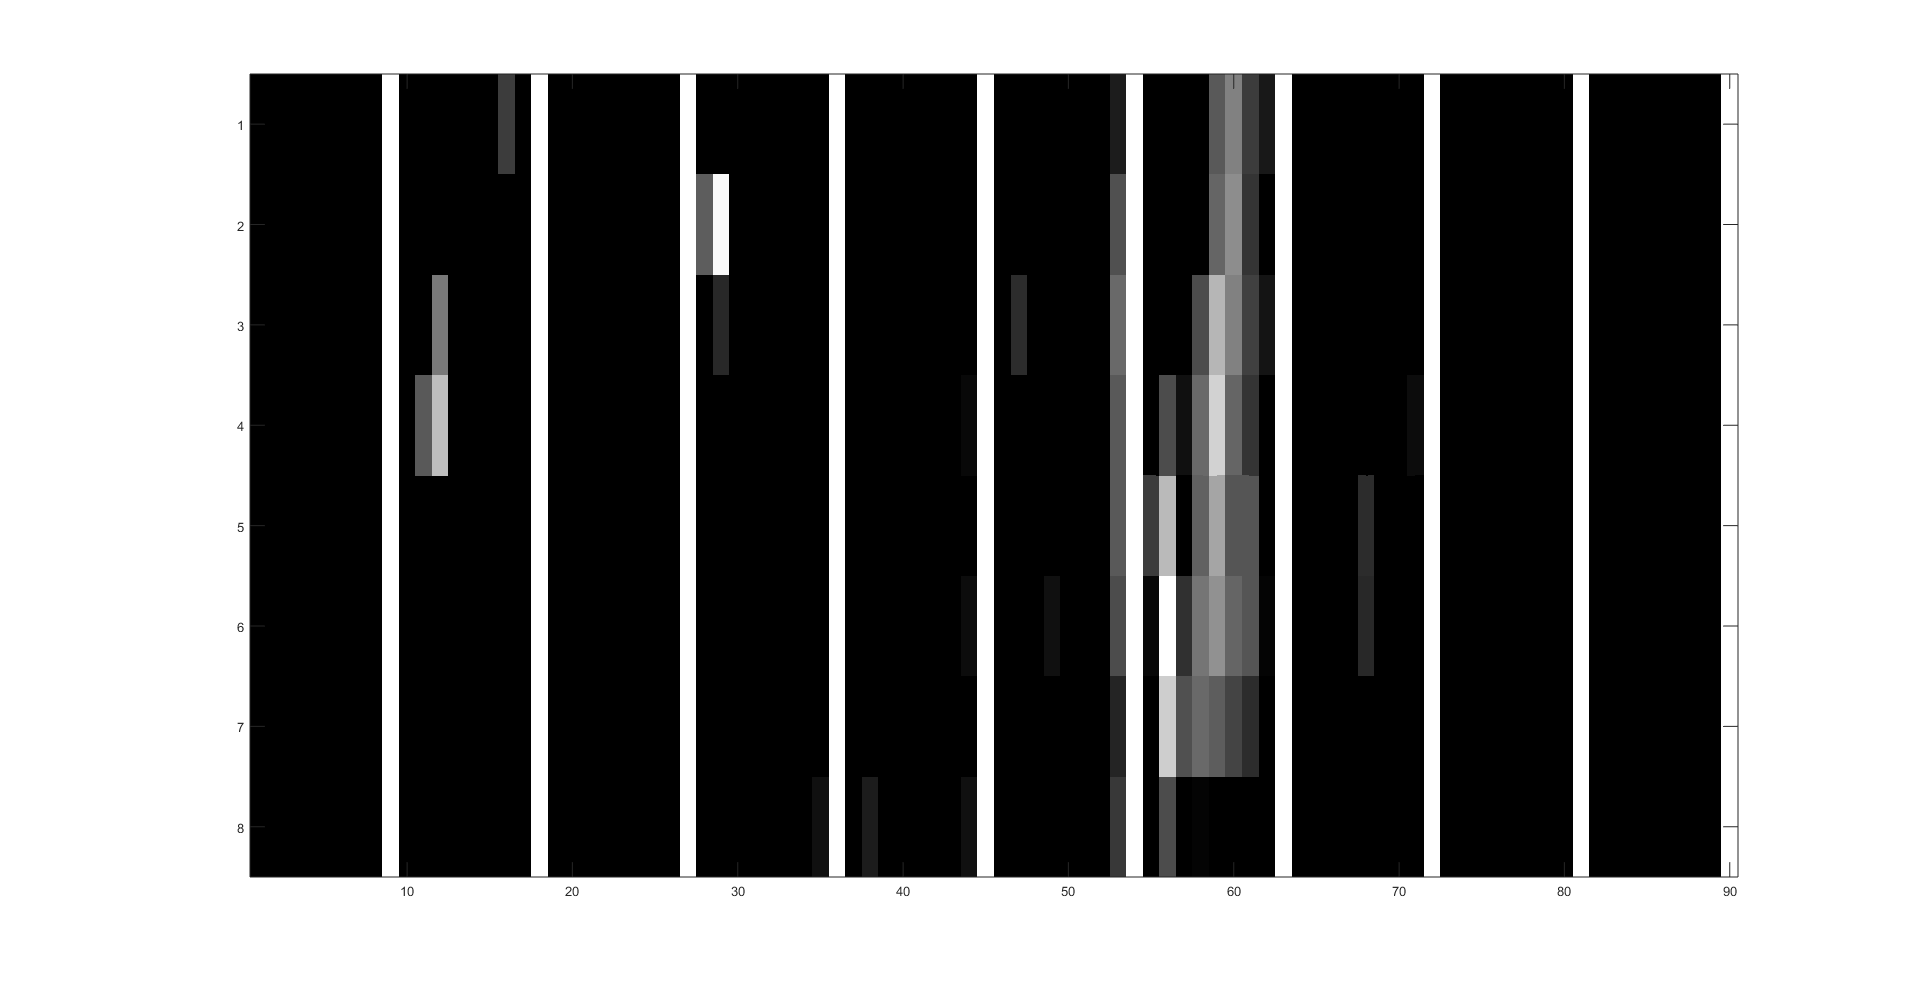
\includegraphics[width=\textwidth]{layer/13}
\end{figure}

\begin{figure}[h!]
  \caption{Layer 14 Output}
  \centering
    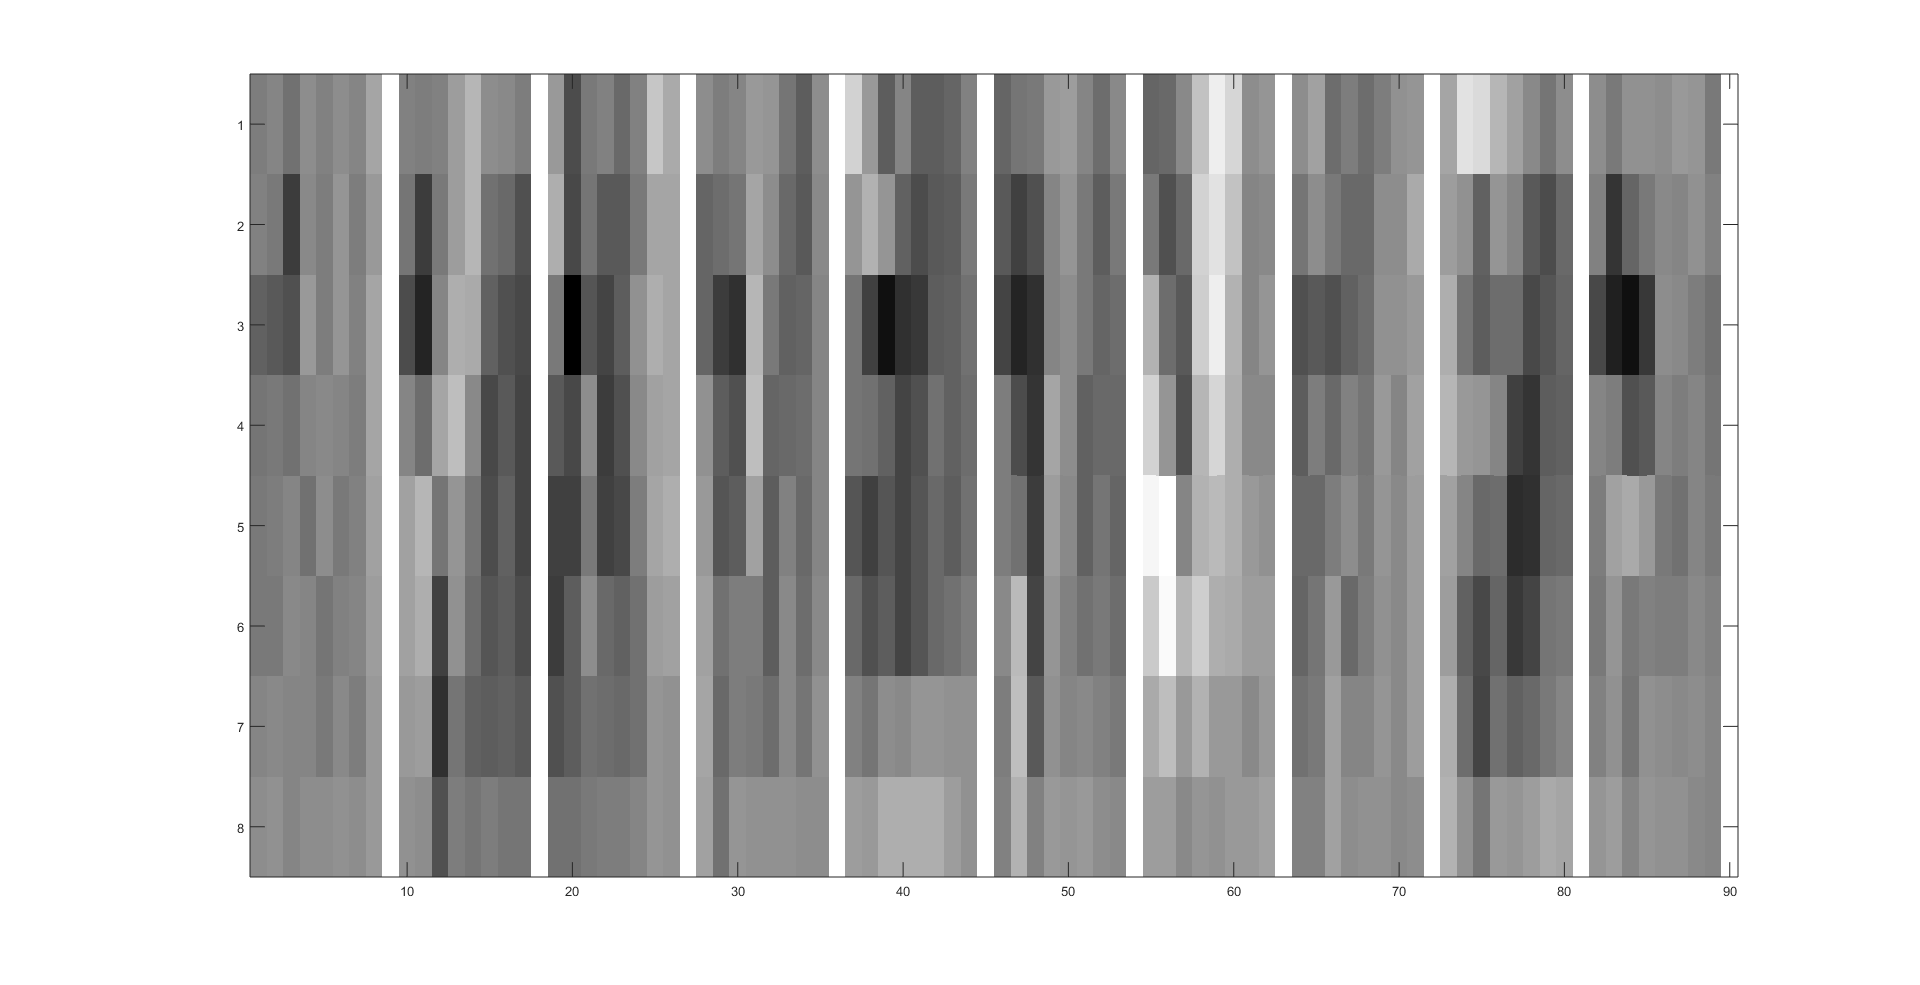
\includegraphics[width=\textwidth]{layer/14}
\end{figure}

\begin{figure}[h!]
  \caption{Layer 15 Output}
  \centering
    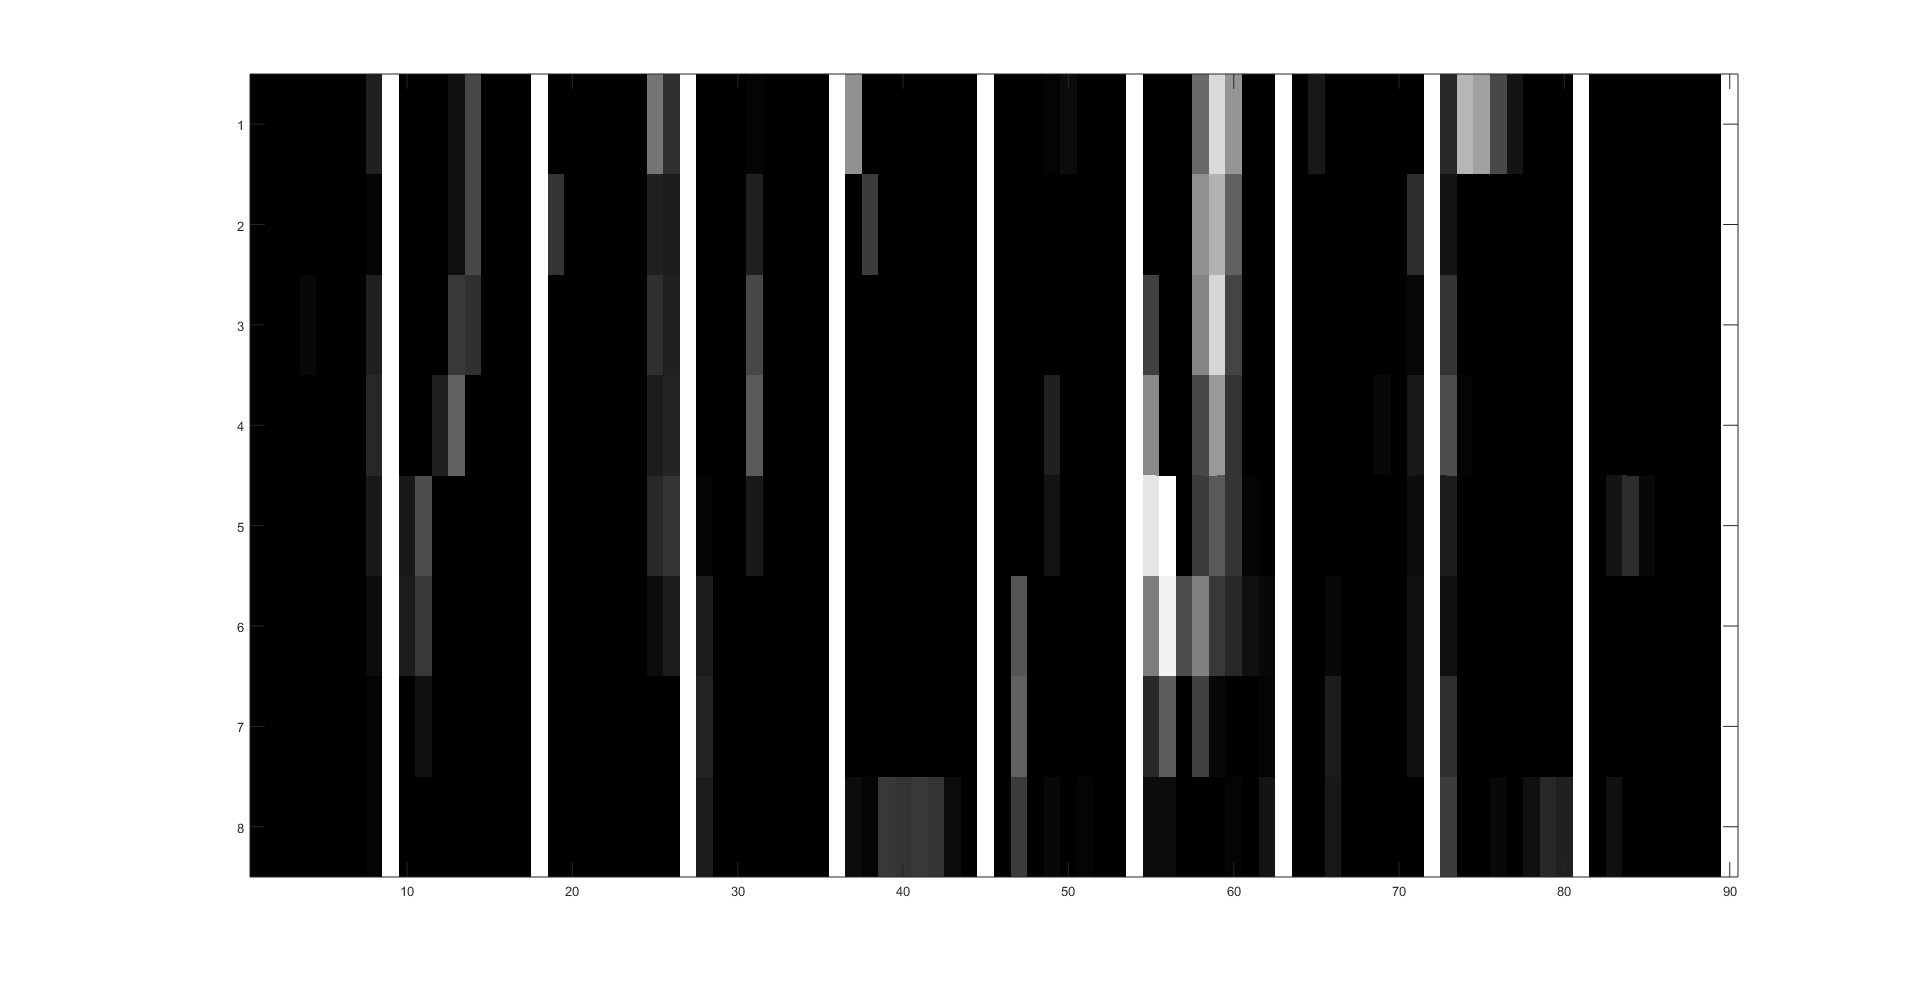
\includegraphics[width=\textwidth]{layer/15}
\end{figure}

\begin{figure}[h!]
  \caption{Layer 16 Output}
  \centering
    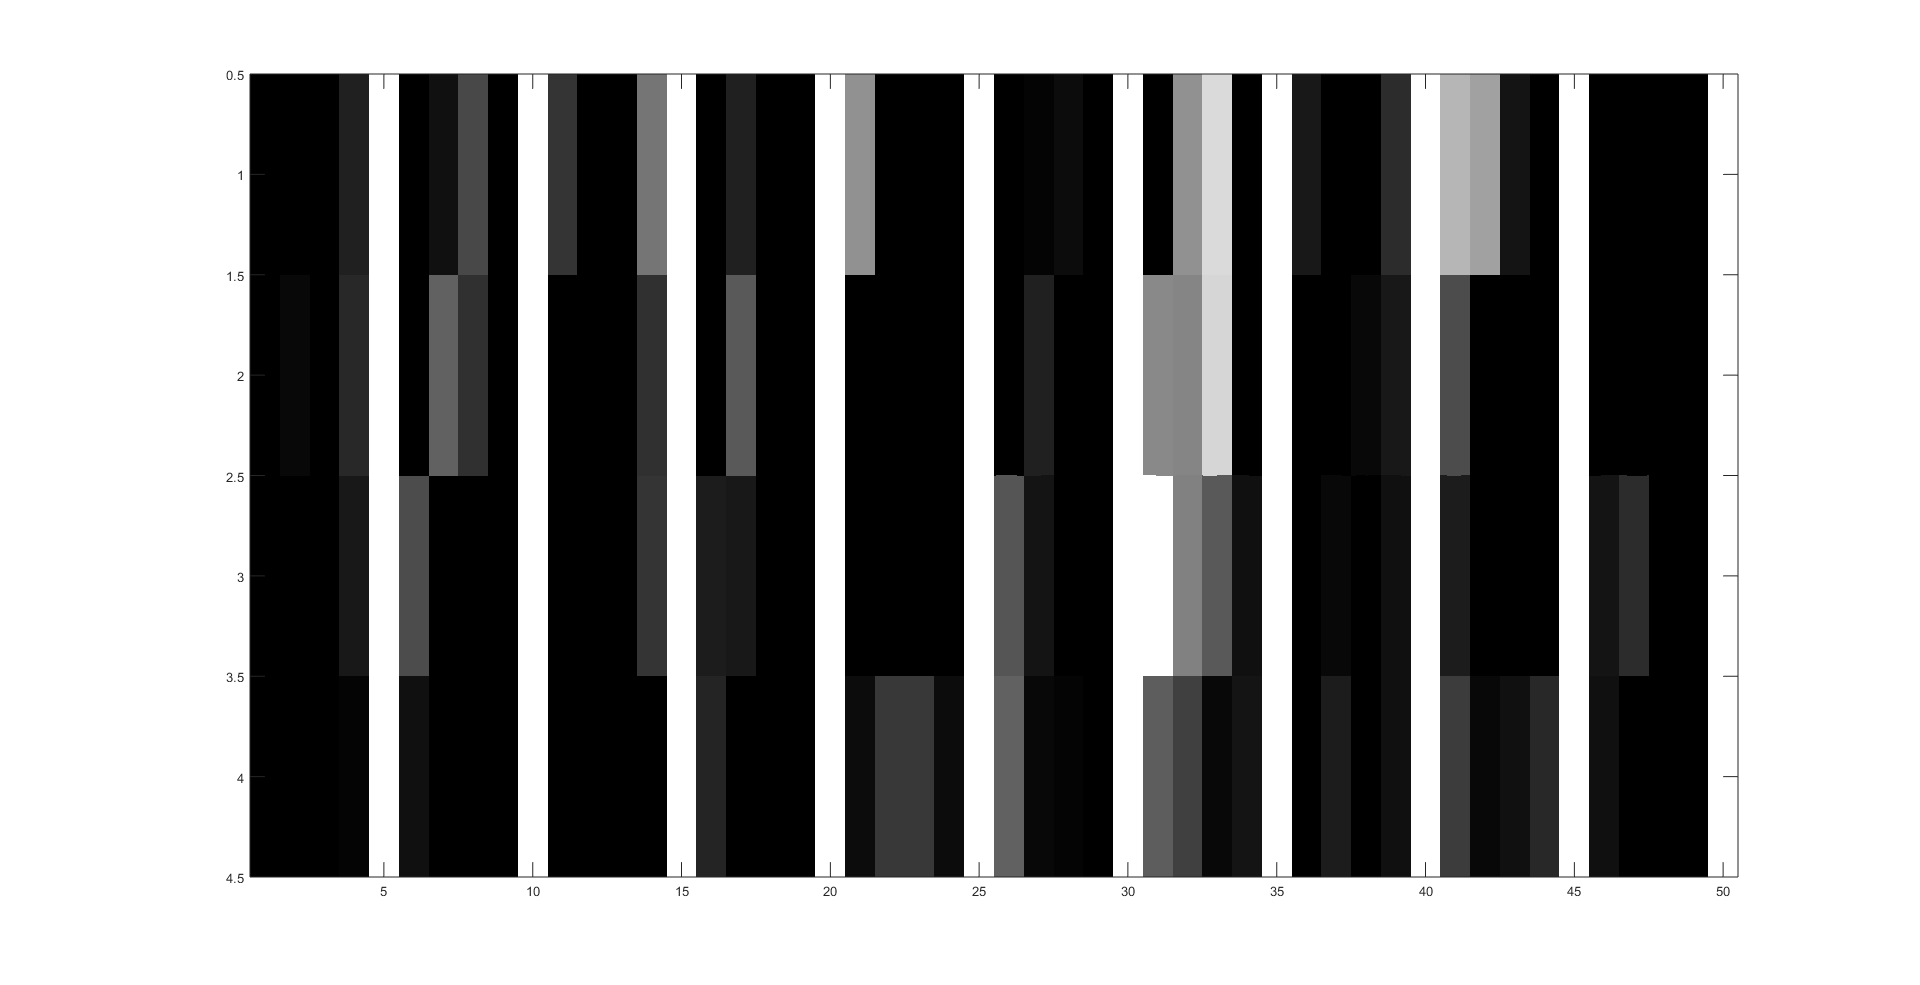
\includegraphics[width=\textwidth]{layer/16}
\end{figure}

\begin{figure}[h!]
  \caption{Layer 17 Output}
  \centering
    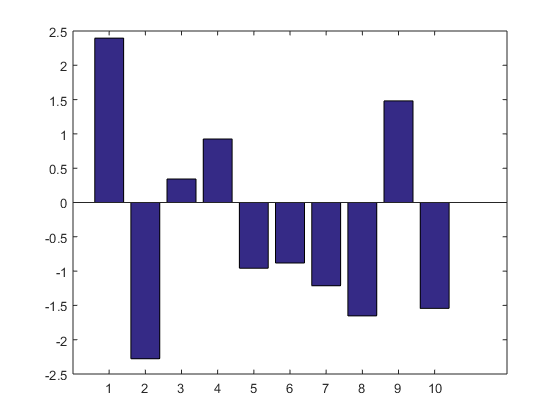
\includegraphics[width=0.75\textwidth]{layer/17}
\end{figure}

\begin{figure}[h!]
  \caption{Layer 18 Output}
  \centering
    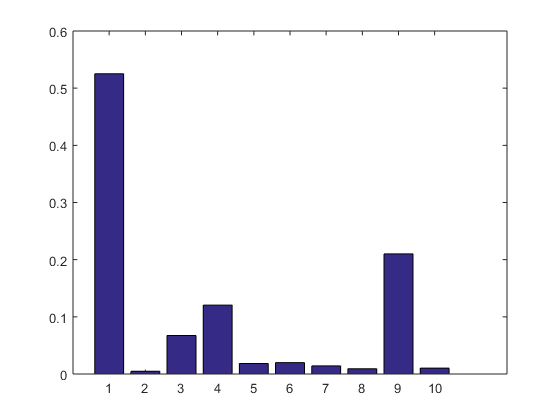
\includegraphics[width=0.75\textwidth]{layer/18}
\end{figure}


\end{appendices}

\end{document}